\documentclass[aspectratio=169]{beamer}
\usetheme{AnnArbor}
\usecolortheme{seahorse}
\useinnertheme{rounded}
\usefonttheme{structurebold}
% ──── Packages ────
\usepackage[utf8]{vietnam}
\usepackage[vietnamese]{babel}
\usepackage{amsmath,amsxtra,amsfonts,amssymb,latexsym,amscd,amsthm,nccmath,listings,mathtools,inputenc, hyperref, geometry, graphicx}
\usepackage[most]{tcolorbox}
\usepackage[T1]{fontenc}
\usefonttheme{serif}
\setbeamertemplate{blocks}[rounded]
\setcounter{section}{-1}
\setlength{\columnseprule}{0.05pt}
\def\columnseprulecolor{\color{black}}

% ──── Comment Filter Settings ────
\usepackage{comment}
\excludecomment{essayonly}
\includecomment{slidesonly}
\excludecomment{scriptonly}
\def\mytitle{Thuật toán điểm cận biên tăng tốc có sai số}
\def\myshorttitle{Đề tài 10}
\def\mygroup{Nhóm 10}
\def\mymembers{
    Nguyễn Hoàng Tú -- MSSV: 23110220\\
    \vspace{3pt}
    Bùi Công Hoàng Vũ -- MSSV: 23110223\\
    \vspace{3pt}
    Huỳnh Trung Kiên -- MSSV: 22110091\\
    \vspace{3pt}
    Nguyễn Ngọc Diễm Quỳnh -- MSSV: 21110167
}
\def\myshortschool{HCMUS}
\def\mylongschool{ĐHKH--TN}
\def\mysupervisor{TS. Nguyễn Đăng Khoa}
\def\mylongdate{Ngày 24 tháng 7 năm 2026}
\def\myshortdate{24/07/2026}
% ──── Custom Preamble ────
\renewcommand{\baselinestretch}{0.8} % giãn dòng

\newcommand{\Hil}{\mathcal{H}}
\DeclareMathOperator{\dom}{dom}
\DeclareMathOperator{\diam}{diam}
\newcommand{\eps}{\varepsilon}
\DeclarePairedDelimiter{\iprod}{\langle}{\rangle}
\DeclarePairedDelimiter{\norm}{\|}{\|}
\providecommand{\citep}[1]{\cite{#1}}
\providecommand{\citealp}[1]{\cite{#1}}
\newcommand{\R}{\mathbb{R}}
\newcommand{\N}{\mathbb{N}}
\newcommand{\prox}{\operatorname{prox}}
\newcommand{\argmin}{\operatorname*{argmin}}
\newcommand{\order}{\mathcal{O}}
\renewcommand{\max}[1]{\operatorname*{max}\left\{#1\right\}}
\newcommand{\Set}[1]{\left\{#1\right\}}
\newcommand{\autotag}[1]{\stepcounter{equation}\tag{\theequation}\label{#1}}
\newcommand{\paragraph}[1]{\par\noindent\textbf{#1}\par}

\let\theorem\relax
\let\endtheorem\relax
\let\lemma\relax
\let\endlemma\relax
\let\corollary\relax
\let\endcorollary\relax
\let\definition\relax
\let\enddefinition\relax
\let\example\relax
\let\endexample\relax

\newenvironment{theorem}{\par\medskip\noindent\textbf{Định lý.}\ }{\par\medskip}
\newenvironment{lemma}{\par\medskip\noindent\textbf{Bổ đề.}\ }{\par\medskip}
\newenvironment{corollary}{\par\medskip\noindent\textbf{Hệ quả.}\ }{\par\medskip}
\newenvironment{definition}{\par\medskip\noindent\textbf{Định nghĩa.}\ }{\par\medskip}
\newenvironment{example}{\par\medskip\noindent\textbf{Ví dụ.}\ }{\par\medskip}
\newenvironment{proposition}{\par\medskip\noindent\textbf{Mệnh đề.}\ }{\par\medskip}
\newenvironment{algorithmenv}{\par\medskip\noindent\textbf{Thuật toán.}\ }{\par\medskip}
\newenvironment{remark}{\par\medskip\noindent\textbf{Nhận xét.}\ }{\par\medskip}

\AtBeginEnvironment{figure}{\framebreak}
\AtEndEnvironment{figure}{\framebreak}

\let\realsection\section
\let\realsubsection\subsection
\let\realsubsubsection\subsubsection
\renewcommand{\subsection}{\realsubsubsection}
\renewcommand{\section}{\realsubsection}
\newcommand{\chapter}{\realsection}

\AtBeginSection[]
{
	\begin{frame}[plain]\large
		\textbf{\tableofcontents[
            currentsection,
            hideothersubsections]}
	\end{frame}
}
\AtBeginSubsection[]
{
	\begin{frame}[plain]\large
		\textbf{\tableofcontents[
            currentsection,
            hideothersubsections,
            subsectionstyle=show/shaded/hide,
            subsubsectionstyle=show/show/hide/hide]}
	\end{frame}
}

% ──── Metadata ────
\title[\myshorttitle]{\textbf{\mytitle}}
\subtitle{\small Dựa trên bài báo: \textit{Inexact and Accelerated Proximal Point Algorithms} (S. Salzo \& S. Villa, 2012)\normalsize}
\author[\mygroup]{
    \textbf{\mygroup} \\
    \vspace{9pt} % Tạo khoảng cách giữa tên nhóm và thành viên
    \mymembers
}
\institute[\myshortschool]{
    \textbf{Giảng viên hướng dẫn: }\mysupervisor\\
    \vspace{14.17pt}
    \mylongschool
}
\date[\myshortdate]{\mylongdate}

% ──── Document ────
\begin{document}
	\nocite{salzovilla2012}
	\frame{\titlepage}
    \chapter{Cơ sở toán học}
    \section{Toán tử gần kề}\label{sec:setting}
    \begin{frame}[allowframebreaks]
    \begin{definition}
Với $\lambda>0$ và $y\in\Hil$, điểm gần kề của $y$ theo hàm $F$ được định nghĩa bởi
\begin{equation}
    \prox_{\lambda F}(y)
    :=
    \argmin_{x\in\Hil}
    \left\{
    \Phi_\lambda(x)
    :=
    F(x)
    +
    \frac1{2\lambda}\norm{x-y}^2
    \right\}.
\end{equation}
\end{definition}

\begin{essayonly}
Do $\Phi_\lambda$ là tổng của một hàm lồi và một hàm toàn phương $1/\lambda$-lồi mạnh, bài toán trên luôn có nghiệm duy nhất. Hơn nữa, điều kiện tối ưu bậc một bài toán lồi cho ta đặc trưng quen thuộc
\end{essayonly}
\begin{equation}
  z = \prox_{\lambda F}(y)
  \iff 0 \in \partial \Phi_\lambda(z)
  \iff \frac{y-z}{\lambda} \in \partial F(z),
  \label{eq:opt-cond}
\end{equation}
\begin{essayonly}
Từ đặc trưng trên suy ra $$\prox_{\lambda F}=(I+\lambda\partial F)^{-1},$$ nghĩa là toán tử gần kề chính là toán tử phân giải của dưới vi phân $\partial F$.
\end{essayonly}
Trên thực tế, việc tính $\prox_{\lambda F}(y)$ tự nó có thể khó không kém việc giải bài toán ban đầu, nên ta cần một khái niệm về xấp xỉ của điểm gần kề. Công cụ thường dùng là $\eps$-dưới vi phân: với $\eps\ge 0$,
\begin{equation}
  \partial_\eps F(z) := \big\{ \xi\in\Hil :
     F(x) \ge F(z) + \iprod{x-z}{\xi} - \eps,\ \forall x\in\Hil \big\}.
  \label{eq:eps-subdiff}
\end{equation}
Khi $\eps=0$, ta thu được dưới vi phân thông thường. Ta có một tính chất cơ bản sau đây
\begin{equation}
  0\in\partial_\eps F(z)
  \iff
  F(z)\le\inf F+\eps.
  \label{eq:eps-subopt}
\end{equation}
\begin{essayonly}
Nói cách khác, điều kiện \textit{$0$ là một $\eps$-dưới gradient tại $z$} tương đương với việc \textit{$z$ là một điểm $\eps$-tối ưu} của bài toán.
\begin{proof}
Theo định nghĩa của $\eps$-dưới vi phân,
\[
0\in\partial_\eps F(z)
\iff
F(x)\ge F(z)-\eps,\qquad\forall x\in\Hil.
\]
Lấy infimum theo $x$ suy ra
\[
\inf F\ge F(z)-\eps,
\iff
F(z)\le\inf F+\eps.
\]
Ngược lại, nếu $F(z)\le\inf F+\eps$ thì với mọi $x\in\Hil$,
\[
F(x)\ge\inf F\ge F(z)-\eps
=
F(z)+\langle x-z,0\rangle-\eps,
\]
nên theo định nghĩa của $\partial_\eps F(z)$,
\[
0\in\partial_\eps F(z).
\]
\end{proof}
\end{essayonly}

\begin{essayonly}
Dựa trên khái niệm $\eps$-dưới vi phân, ta sẽ xét ba mô hình xấp xỉ của điểm gần kề. Cả ba đều thuộc lớp sai số tuyệt đối, nghĩa là tham số sai số $\eps$ được quy định độc lập với vị trí của điểm $y$ cũng như độ lớn của điểm gần kề cần tính.
\end{essayonly}


    \end{frame}
    \section{Xấp xỉ điểm gần kề}
    \begin{frame}[allowframebreaks]
    \begin{definition}[Xấp xỉ loại 1]
Cho $\lambda>0$, $y\in\Hil$ và $\eps\ge0$. Một điểm $z\in\Hil$ được gọi là xấp xỉ loại~1 của $\prox_{\lambda F}(y)$ với độ chính xác $\eps$, ký hiệu
\[
z\approx_1\prox_{\lambda F}(y)
\]
nếu
\begin{equation}
0\in\partial_{\eps^2/(2\lambda)}\Phi_\lambda(z).
\tag{AT1}
\label{eq:AT1}
\end{equation}
\end{definition}

\begin{essayonly}
Đây là khái niệm xấp xỉ tự nhiên nhất khi điểm gần kề được tính bằng một thuật toán cực tiểu hóa hàm phụ
\[
\Phi_\lambda(x)
=
F(x)+\frac1{2\lambda}\norm{x-y}^2.
\]
Thật vậy, áp dụng \eqref{eq:eps-subopt} cho $\Phi_\lambda$, điều kiện
\eqref{eq:AT1} tương đương với
\[
\Phi_\lambda(z)
\le
\Phi_\lambda^*
+
\frac{\eps^2}{2\lambda}
\]
trong đó $\Phi_\lambda^*$ là giá trị tối ưu của bài toán gần kề. Nói cách khác, $z$ chỉ cần cực tiểu hóa bài toán con với sai số hàm mục tiêu không vượt quá $\eps^2/(2\lambda)$. Đây cũng chính là tiêu chí dừng thường gặp trong các thuật toán giải bài toán gần kề.

Điều kiện trên không chỉ bảo đảm sai số về giá trị hàm mục tiêu mà còn cho phép kiểm soát trực tiếp khoảng cách từ nghiệm gần đúng đến điểm gần kề chính xác, như kết quả sau đây.
\end{essayonly}

\begin{proposition}
\label{prop:type1-bound}
Nếu
\[
z\approx_1\prox_{\lambda F}(y)\quad\text{với $\eps$-chính xác}
\]
thì
\[
z\in\dom F
\qquad
\norm{z-\prox_{\lambda F}(y)}
\le
\eps.
\]
\end{proposition}

\begin{essayonly}
\begin{proof}
Đặt
\[
x^*=\prox_{\lambda F}(y).
\]
Do $\Phi_\lambda$ là hàm $1/\lambda$-lồi mạnh và $x^*$ là điểm cực tiểu của nó, bất đẳng thức lồi mạnh cho
\[
\Phi_\lambda(z)-\Phi_\lambda(x^*)
\ge
\frac1{2\lambda}\norm{z-x^*}^2.
\]

Mặt khác, từ \eqref{eq:AT1} và hệ quả \eqref{eq:eps-subopt} suy ra
\[
\Phi_\lambda(z)
\le
\Phi_\lambda^*
+
\frac{\eps^2}{2\lambda}
=
\Phi_\lambda(x^*)
+
\frac{\eps^2}{2\lambda}.
\]
Kết hợp hai bất đẳng thức trên, ta được
\[
\frac1{2\lambda}\norm{z-x^*}^2
\le
\frac{\eps^2}{2\lambda}
\;\text{hay}\;
\norm{z-x^*}\le\eps.
\]
Đặc biệt,
$\Phi_\lambda(z)<+\infty$, nên $F(z)<+\infty$, tức
$z\in\dom F$.
\end{proof}
\end{essayonly}

\begin{definition}[Xấp xỉ loại 2]
Cho $\lambda>0$, $y\in\Hil$ và $\eps\ge0$. Một điểm $z\in\Hil$ được gọi là xấp xỉ loại~2 của $\prox_{\lambda F}(y)$ với độ chính xác $\eps$, ký hiệu
\[
z\approx_2\prox_{\lambda F}(y),
\]
nếu
\begin{equation}
\frac{y-z}{\lambda}
\in
\partial_{\eps^2/(2\lambda)}F(z).
\tag{AT2}
\label{eq:AT2}
\end{equation}
\end{definition}

So với điều kiện tối ưu chính xác \eqref{eq:opt-cond}, định nghĩa trên chỉ thay dưới vi phân $\partial F(z)$ bằng $\eps^2/(2\lambda)$-dưới vi phân của $F$ tại $z$. Vì thế, xấp xỉ loại~2 có thể được xem như một dạng mở rộng của điều kiện tối ưu cho toán tử gần kề.

\begin{definition}[Xấp xỉ loại 3]
Cho $\lambda>0$, $y\in\Hil$ và $\eps\ge0$. Một điểm
$z\in\Hil$ được gọi là xấp xỉ loại~3 của
$\prox_{\lambda F}(y)$ với độ chính xác $\eps$, ký hiệu
\[
z\approx_3\prox_{\lambda F}(y),
\]
nếu
\begin{equation}
d\bigl(0,\partial\Phi_\lambda(z)\bigr)
\le
\frac{\eps}{\lambda}.
\tag{AT3}
\label{eq:AT3}
\end{equation}
\end{definition}
Điểm nổi bật của xấp xỉ loại~3 là nó có một cách diễn giải rất trực quan. Thật vậy, từ công thức
\[
\partial\Phi_\lambda(z)
=
\partial F(z)
+
\frac{z-y}{\lambda},
\]
điều kiện \eqref{eq:AT3} tương đương với sự tồn tại một vectơ
$e\in\Hil$ thỏa $\norm e\le\eps$ sao cho
\[
\frac{y+e-z}{\lambda}
\in
\partial F(z).
\]
Kết hợp với đặc trưng của toán tử gần kề trong
\eqref{eq:opt-cond}, ta thu được
\begin{equation}
z\approx_3\prox_{\lambda F}(y)\quad\text{với $\eps$-chính xác}
\iff
\exists\,e\in\Hil,\;
\norm e\le\eps,\;
z=\prox_{\lambda F}(y+e).
\label{eq:AT3-equiv}
\end{equation}

\begin{essayonly}
Nói cách khác, một xấp xỉ loại~3 chính là điểm gần kề chính xác ứng với một đầu vào bị nhiễu. Cách diễn giải này đặc biệt thuận tiện khi phân tích ảnh hưởng của nhiễu hoặc khi chủ động đưa sai số vào các mô phỏng số.
\end{essayonly}

\begin{remark}
Khi $\varepsilon=0$, cả ba khái niệm xấp xỉ đều trở về điều kiện tối ưu chính xác của toán tử gần kề. Thật vậy,
\[
\begin{aligned}
\text{(AT1)}&\iff 0\in\partial\Phi_\lambda(z),\\
\text{(AT2)}&\iff \frac{y-z}{\lambda}\in\partial F(z),\\
\text{(AT3)}&\iff d(0,\partial\Phi_\lambda(z))=0
           \iff 0\in\partial\Phi_\lambda(z).
\end{aligned}
\]
Do đặc trưng \eqref{eq:opt-cond}, cả ba điều kiện trên đều tương đương với
\[
z=\operatorname{prox}_{\lambda F}(y).
\]
Vì vậy, ba mô hình xấp xỉ được trình bày ở trên đều là các mở rộng tự nhiên của khái niệm điểm gần kề chính xác.
\end{remark}

    \end{frame}
    \section{Mối quan hệ giữa các xấp xỉ}
    \begin{frame}[allowframebreaks]
    \begin{essayonly}
Ba khái niệm xấp xỉ vừa giới thiệu không tồn tại một cách độc lập mà có mối liên hệ chặt chẽ với nhau. Để làm rõ mối quan hệ này, trước hết ta khai triển $\eps$-dưới vi phân của hàm gần kề
\[
\Phi_\lambda
=
F+\frac1{2\lambda}\norm{\cdot-y}^2.
\]

Theo công thức dưới vi phân của tổng đối với $\eps$-dưới vi phân, ta có
\[
\partial_{\eps^2/(2\lambda)}\Phi_\lambda(z)
=
\bigcup_{\substack{\eps_1,\eps_2\ge0\\
\eps_1+\eps_2\le\eps^2/(2\lambda)}}
\left(
\partial_{\eps_1}F(z)
+
\Bigl\{
\frac{z-y+e}{\lambda}:
\frac{\norm e^2}{2\lambda}\le\eps_2
\Bigr\}
\right).
\]

Từ công thức trên, điều kiện của xấp xỉ loại~1 có thể được phát biểu dưới nhiều dạng tương đương.
\end{essayonly}
\begin{lemma}
\label{lem:equiv-AT1}
Các mệnh đề sau tương đương:
\begin{enumerate}
  \item $z\approx_1 \prox_{\lambda F}(y)\quad\text{với $\eps$-chính xác}$
  \item tồn tại $\eps_1,\eps_2\ge0$ với $\eps_1+\eps_2\le\eps^2/2\lambda$, tồn tại $\xi\in\partial_{\eps_1}F(z)$ và $e\in\Hil$ với $\norm{e}^2/2\lambda \le \eps_2$, sao cho $\lambda\xi+(z-y+e)=0$;
  \item tồn tại $\eps_1,\eps_2\ge0$ với $\eps_1^2+\eps_2^2\le\eps^2$, tồn tại $e\in\Hil$ với $\norm{e}\le\eps_2$, sao cho $(y-z+e)/\lambda \in \partial_{\eps_1^2/2\lambda}F(z)$.
\end{enumerate}
\end{lemma}
\begin{essayonly}
\begin{proof}
Trước hết, theo công thức khai triển của $\eps$-dưới vi phân đối với tổng hai hàm lồi,
\[
\partial_{\eps^2/(2\lambda)}\Phi_\lambda(z)
=
\bigcup_{\substack{\varepsilon_1,\varepsilon_2\ge0\\
\varepsilon_1+\varepsilon_2\le\eps^2/(2\lambda)}}
\left(
\partial_{\varepsilon_1}F(z)
+
\Bigl\{
\frac{z-y+e}{\lambda}:
\frac{\norm e^2}{2\lambda}\le\varepsilon_2
\Bigr\}
\right).
\]

Do đó,
\[
0\in\partial_{\eps^2/(2\lambda)}\Phi_\lambda(z)
\]
khi và chỉ khi tồn tại
$\varepsilon_1,\varepsilon_2\ge0$ thỏa
$\varepsilon_1+\varepsilon_2\le\eps^2/(2\lambda)$,
$\xi\in\partial_{\varepsilon_1}F(z)$ và
$e\in\Hil$ với
$\norm e^2/(2\lambda)\le\varepsilon_2$ sao cho
\[
0
=
\xi+\frac{z-y+e}{\lambda}.
\]
Nhân hai vế với $\lambda$ ta được
\[
\lambda\xi+(z-y+e)=0,
\]
đúng với phát biểu (ii). Vì vậy,
\[
\mathrm{(i)}
\Longleftrightarrow
\mathrm{(ii)}.
\]

Tiếp theo, ta chứng minh
\[
\mathrm{(ii)}
\Longleftrightarrow
\mathrm{(iii)}.
\]

Giả sử (ii) đúng. Đặt
\[
\tilde\eps_1=\sqrt{2\lambda\varepsilon_1},
\qquad
\tilde\eps_2=\norm e.
\]
Từ
\[
\varepsilon_1+\varepsilon_2
\le
\frac{\eps^2}{2\lambda},
\qquad
\frac{\norm e^2}{2\lambda}
\le
\varepsilon_2,
\]
suy ra
\[
\tilde\eps_1^2+\tilde\eps_2^2
=
2\lambda\varepsilon_1+\norm e^2
\le
2\lambda(\varepsilon_1+\varepsilon_2)
\le
\eps^2.
\]
Mặt khác, từ
\[
\lambda\xi+(z-y+e)=0
\]
ta có
\[
\xi
=
\frac{y-z-e}{\lambda}
\in
\partial_{\tilde\eps_1^2/(2\lambda)}F(z).
\]
Đổi $e$ thành $-e$ (không làm thay đổi chuẩn của $e$), ta được
\[
\frac{y-z+e}{\lambda}
\in
\partial_{\tilde\eps_1^2/(2\lambda)}F(z),
\]
đúng với phát biểu (iii).

Ngược lại, giả sử (iii) đúng. Đặt
\[
\varepsilon_1=\frac{\eps_1^2}{2\lambda},
\qquad
\varepsilon_2=\frac{\eps_2^2}{2\lambda}.
\]
Điều kiện
\[
\eps_1^2+\eps_2^2\le\eps^2
\]
suy ra
\[
\varepsilon_1+\varepsilon_2
\le
\frac{\eps^2}{2\lambda},
\]
và từ
\[
\frac{y-z+e}{\lambda}
\in
\partial_{\varepsilon_1}F(z)
\]
ta suy ra
\[
\lambda\xi+(z-y-e)=0,
\qquad
\xi=\frac{y-z+e}{\lambda}.
\]
Đổi $e$ thành $-e$ một lần nữa, ta thu được đúng phát biểu (ii).

Vậy ba mệnh đề (i), (ii) và (iii) là tương đương.
\end{proof}
\end{essayonly}

\begin{essayonly}
Bổ đề~\ref{lem:equiv-AT1} cho thấy xấp xỉ loại~1 đóng vai trò là một mô hình tổng quát bao hàm cả xấp xỉ loại~2 và loại~3. Cụ thể, điều kiện tương đương ở Bổ đề~\ref{lem:equiv-AT1}(iii) cho phép tách sai số tổng thể thành hai đại lượng độc lập: một đại lượng bị hấp thụ bởi $\eps$-dưới vi phân của $F$, và đại lượng kia đóng vai trò là nhiễu của điểm tham chiếu. Khi dồn toàn bộ sai số vào một trong hai thành phần này (hai trường hợp cực biên), ta thu được chính xác định nghĩa của xấp xỉ loại~2 và loại~3. Mối liên hệ này được phát biểu chính xác trong các mệnh đề sau.
\end{essayonly}
\begin{proposition}
\label{prop:relations}
Các khẳng định sau đúng:
\begin{enumerate}
  \item $z\approx_2\prox_{\lambda F}(y)\quad\text{với $\eps$-chính xác}$ $\implies$ $z\approx_1\prox_{\lambda F}(y)\quad\text{với $\eps$-chính xác}$;
  \item $z\approx_3\prox_{\lambda F}(y)\quad\text{với $\eps$-chính xác}$ $\implies$ $z\approx_1\prox_{\lambda F}(y)\quad\text{với $\eps$-chính xác}$;
  \item Nếu thêm giả thiết $F$ lồi mạnh với hệ số $\mu>0$ thì
        $z\approx_1\prox_{\lambda F}(y)\quad\text{với $\eps$-chính xác}$ $\implies$ $z\approx_2\prox_{\lambda F}(y)\quad\text{với $\eps\sqrt{(\lambda\mu+1)/\lambda\mu}$-chính xác}$; nói riêng, nếu $\lambda\ge 1/\mu$ thì độ chính xác có thể lấy là $\eps\sqrt{2}$.
\end{enumerate}
\end{proposition}
\begin{essayonly}
\begin{proof}

1) Giả sử
$
z\approx_2\prox_{\lambda F}(y)\quad\text{với $\eps$-chính xác}
$. Theo định nghĩa,
\[
\frac{y-z}{\lambda}
\in
\partial_{\eps^2/(2\lambda)}F(z).
\]
Trong Bổ đề~\ref{lem:equiv-AT1}(iii), chỉ cần chọn
\[
\eps_1=\eps,\qquad
\eps_2=0,\qquad
e=0.
\]
Khi đó
\[
\eps_1^2+\eps_2^2=\eps^2,
\]
và điều kiện của (iii) được thỏa mãn. Suy ra
$
z\approx_1\prox_{\lambda F}(y)\quad\text{với $\eps$-chính xác}
$.

\medskip

2) Giả sử
$
z\approx_3\prox_{\lambda F}(y)\quad\text{với $\eps$-chính xác}
$. Theo công thức tương đương \eqref{eq:AT3-equiv}, tồn tại
$e\in\Hil$ với
$\norm e\le\eps$ sao cho
\[
\frac{y-z+e}{\lambda}
\in
\partial F(z).
\]
Do
\[
\partial F(z)=\partial_0F(z),
\]
trong Bổ đề~\ref{lem:equiv-AT1}(iii) ta chỉ cần chọn
\[
\eps_1=0,\qquad
\eps_2=\eps.
\]
Khi đó điều kiện của (iii) được thỏa mãn, và do đó
$
z\approx_1\prox_{\lambda F}(y)\quad\text{với $\eps$-chính xác}
$.

\medskip

3) Giả sử
$
z\approx_1\prox_{\lambda F}(y)\quad\text{với $\eps$-chính xác}
$. Theo Định nghĩa~\ref{eq:AT1} và hệ quả
\eqref{eq:eps-subopt},
\[
\Phi_\lambda(x)
\ge
\Phi_\lambda(z)
-
\frac{\eps^2}{2\lambda},
\qquad
\forall x\in\Hil.
\]
Viết lại theo định nghĩa của $\Phi_\lambda$, ta được
\[
F(x)
+
\frac1{2\lambda}\norm{x-y}^2
\ge
F(z)
+
\frac1{2\lambda}\norm{z-y}^2
-
\frac{\eps^2}{2\lambda}.
\]
Khai triển
\[
\norm{x-y}^2
=
\norm{x-z}^2
+
2\langle x-z,z-y\rangle
+
\norm{z-y}^2,
\]
rút gọn hai vế, suy ra
\[
F(x)
\ge
F(z)
+
\frac1\lambda
\langle x-z,y-z\rangle
-
\frac1{2\lambda}\norm{x-z}^2
-
\frac{\eps^2}{2\lambda},
\qquad
\forall x\in\Hil.
\]

Ta khai thác giả thiết $F$ lồi mạnh với hệ số $\mu$. Với
$\theta\in(0,1]$, đặt
\[
x_\theta
=
\theta x+(1-\theta)z.
\]
Theo tính lồi mạnh,
\[
F(x_\theta)
\le
\theta F(x)
+
(1-\theta)F(z)
-
\frac\mu2
\theta(1-\theta)
\norm{x-z}^2.
\]
Mặt khác, áp dụng bất đẳng thức trên cho $x_\theta$ thay cho $x$,
\[
F(x_\theta)
\ge
F(z)
+
\frac{\theta}{\lambda}
\langle x-z,y-z\rangle
-
\frac{\theta^2}{2\lambda}
\norm{x-z}^2
-
\frac{\eps^2}{2\lambda}.
\]
Kết hợp hai bất đẳng thức này, rút gọn và chia cho $\theta$, ta thu được
\[
F(x)
\ge
F(z)
+
\left\langle
x-z,
\frac{y-z}{\lambda}
\right\rangle
+
\frac{1}{2\lambda}
\bigl(
\lambda\mu(1-\theta)-\theta
\bigr)
\norm{x-z}^2
-
\frac{\eps^2}{2\lambda\theta}.
\]

Nếu chọn
\[
\theta
\le
\frac{\lambda\mu}{1+\lambda\mu},
\]
thì
\[
\lambda\mu(1-\theta)-\theta\ge0,
\]
nên số hạng bậc hai không âm và có thể bỏ đi. Khi đó
\[
F(x)
\ge
F(z)
+
\left\langle
x-z,
\frac{y-z}{\lambda}
\right\rangle
-
\frac{\eps^2}{2\lambda\theta},
\qquad
\forall x\in\Hil,
\]
hay
\[
\frac{y-z}{\lambda}
\in
\partial_{\eps^2/(2\lambda\theta)}F(z).
\]
Chọn
\[
\theta
=
\frac{\lambda\mu}{1+\lambda\mu},
\]
ta thu được
\[
\frac{\eps}{\sqrt{\theta}}
=
\eps
\sqrt{\frac{1+\lambda\mu}{\lambda\mu}},
\]
chính là độ chính xác trong phát biểu.

Nếu thêm
\[
\lambda\ge\frac1\mu,
\]
thì
\[
\frac12
\le
\frac{\lambda\mu}{1+\lambda\mu},
\]
nên có thể chọn đơn giản $\theta=\frac12$, từ đó suy ra độ chính xác
$\eps\sqrt2$.

\end{proof}
\end{essayonly}

\begin{essayonly}
Mệnh đề~\ref{prop:relations} cho thấy xấp xỉ loại~1 đóng vai trò như một khái niệm trung tâm trong ba loại xấp xỉ đang xét. Một mặt, mọi xấp xỉ loại~2 và loại~3 đều tự động là xấp xỉ loại~1 với cùng mức sai số. Mặt khác, khi $F$ lồi mạnh, một xấp xỉ loại~1 cũng có thể được chuyển thành xấp xỉ loại~2 với sự suy giảm độ chính xác chỉ bởi một hằng số nhân.
\end{essayonly} 


    \end{frame}
    \section{Ví dụ: Phép chiếu lên một tập lồi}\label{sec:example-projection}
    \begin{frame}[allowframebreaks]
    Một trường hợp đặc biệt giúp minh họa rõ ý nghĩa của ba khái niệm xấp xỉ là khi
\[
F=\iota_C,
\]
trong đó $\iota_C$ là hàm chỉ báo của một tập lồi đóng
$C\subset\Hil$, tức
\[
\iota_C(x)=
\begin{cases}
0, & x\in C,\\
+\infty, & x\notin C.
\end{cases}
\]
Khi đó bài toán điểm gần kề trở thành bài toán chiếu trực giao lên $C$, vì
\[
\prox_{\lambda F}=P_C,
\]
không phụ thuộc vào tham số $\lambda$.
\begin{essayonly}
Do đó, ba khái niệm xấp xỉ của điểm gần kề có thể được diễn giải hoàn toàn bằng hình học, giúp thấy rõ sự khác biệt giữa chúng.
\end{essayonly}

\paragraph{Xấp xỉ loại 1.}
Từ định nghĩa của xấp xỉ loại~1 và tính chất của phép chiếu trực giao, ta suy ra
\begin{equation}
  z\approx_1 P_C(y)\quad\text{với $\eps$-chính xác}
  \iff
  z\in C
  \text{ và }
  \norm{z-y}^2
  \le
  d(y,C)^2+\eps^2.
  \label{eq:proj-type1}
\end{equation}

\begin{figure}[H]
    \centering
    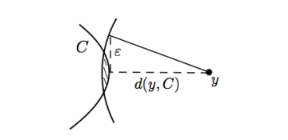
\includegraphics[width=0.5\linewidth]{figures/proj-type1.png}
    \caption{Minh họa xấp xỉ loại~1. Điểm $z$ chỉ cần nằm trong phần tô đậm, tức giao của tập $C$ với hình cầu tâm $y$ có bán kính $\sqrt{d(y,C)^2+\eps^2}$. Vì vậy, $z$ không nhất thiết phải nằm gần điểm chiếu $P_C(y)$.}
    \label{fig:loai_1}
\end{figure}

\begin{essayonly}
Nói cách khác, thay vì yêu cầu $z$ phải là hình chiếu chính xác của $y$ lên $C$, ta chỉ đòi hỏi khoảng cách từ $y$ đến $z$ không vượt quá khoảng cách tối ưu $d(y,C)$ quá một lượng $\eps$. Vì vậy, tập các điểm xấp xỉ loại~1 chính là giao của tập $C$ với hình cầu tâm $y$ có bán kính $\sqrt{d(y,C)^2+\eps^2}$.
\end{essayonly}

\paragraph{Xấp xỉ loại 2.}

Trong trường hợp $F=\iota_C$, điều kiện \eqref{eq:AT2} tương đương với
\begin{equation}
  z\approx_2 P_C(y)\quad\text{với $\eps$-chính xác}
  \iff
  z\in C
  \text{ và }
  \iprod{x-z}{y-z}
  \le
  \frac{\eps^2}{2},
  \quad \forall x\in C.
  \label{eq:proj-type2}
\end{equation}

\begin{essayonly}
Điều kiện trên có thể được hiểu như một sự nới lỏng của đặc trưng hình học đối với phép chiếu trực giao. Điểm chiếu chính xác
$P_C(y)$ được đặc trưng bởi
\[
\iprod{x-P_C(y)}{y-P_C(y)}\le0,
\qquad \forall x\in C,
\]
nghĩa là toàn bộ tập lồi $C$ nằm trong một nửa không gian được xác định bởi siêu phẳng tiếp xúc với $C$ tại $P_C(y)$.

Đối với xấp xỉ loại~2, bất đẳng thức trên được thay bằng
\[
\iprod{x-z}{y-z}\le\frac{\eps^2}{2},
\]
cho phép toàn bộ tập $C$ vượt qua siêu phẳng tiếp xúc một lượng hữu hạn phụ thuộc vào $\eps$. Cụ thể, $C$ chỉ cần nằm trong nửa không gian giới hạn bởi siêu phẳng affine
\[
h_\eps:
\Big\langle
x-z,\,
\frac{y-z}{\norm{y-z}}
\Big\rangle
=
\frac{\eps^2}{2\norm{y-z}},
\]
là siêu phẳng vuông góc với vectơ $y-z$ và song song với siêu phẳng tiếp xúc chính xác. So với trường hợp $\eps=0$, siêu phẳng này được tịnh tiến theo hướng từ $z$ tới $y$ một khoảng
\[
\frac{\eps^2}{2\norm{y-z}}.
\]
\end{essayonly}
\begin{figure}[H]
    \centering
    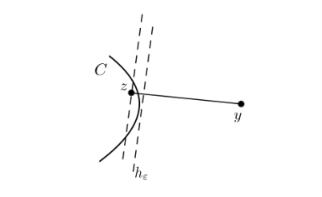
\includegraphics[width=0.5\linewidth]{figures/proj-type2.png}
    \caption{Minh họa xấp xỉ loại 2. Siêu phẳng $h_0$ là siêu phẳng đỡ chính xác tại $z$, còn $h_\varepsilon$ là siêu phẳng song song thu được bằng cách tịnh tiến $h_0$ về phía $y$ một khoảng $\varepsilon^2/(2\|y-z\|)$. Điều kiện \eqref{eq:proj-type2} yêu cầu toàn bộ tập lồi $C$ vẫn nằm trong nửa không gian giới hạn bởi $h_\varepsilon$.}
\label{fig:type2}
\end{figure}

\paragraph{Xấp xỉ loại 3.}
Theo đặc trưng \eqref{eq:AT3-equiv}, xấp xỉ loại~3 của phép chiếu được mô tả bởi
\begin{equation}
  z\approx_3 P_C(y)\quad\text{với $\eps$-chính xác}
  \iff
  z=P_C(y+e),\qquad \norm{e}\le\eps.
  \label{eq:proj-type3}
\end{equation}

\begin{essayonly}
Nói cách khác, thay vì làm tròn trực tiếp điểm chiếu, ta cho phép điểm đầu vào $y$ chịu một nhiễu có chuẩn không vượt quá $\eps$, rồi thực hiện phép chiếu chính xác. Vì vậy, mọi xấp xỉ loại~3 đều là ảnh chiếu của một điểm nằm trong hình cầu tâm $y$, bán kính $\eps$.
\end{essayonly}

\begin{figure}[H]
    \centering
    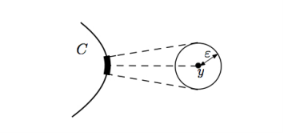
\includegraphics[width=0.5\linewidth]{figures/proj-type3.png}
    \caption{Xấp xỉ loại~3: các điểm xấp xỉ là ảnh chiếu của các điểm trong hình cầu $B(y,\eps)$, do đó luôn nằm trên biên của $C$.}
    \label{fig:type_3}
\end{figure}

\begin{remark}
Một điểm đáng chú ý là, đối với các tập lồi bị chặn, xấp xỉ loại~3 luôn kéo theo xấp xỉ loại~2. Nói cách khác, nếu một điểm là hình chiếu chính xác của một điểm bị nhiễu không quá $\eps$, thì nó đồng thời cũng thỏa điều kiện siêu phẳng của xấp xỉ loại~2 với một sai số lớn hơn nhưng vẫn được kiểm soát tường minh.

\begin{essayonly}
Cụ thể, nếu
\[
z\approx_3P_C(y)
\quad\text{với độ chính xác }\eps,
\]
thì
\[
z\approx_2P_C(y)
\quad\text{với độ chính xác }
\sqrt{2\,\diam(C)\,\eps}.
\]

Thật vậy, theo đặc trưng của xấp xỉ loại~3 trong
\eqref{eq:proj-type3}, tồn tại một vectơ nhiễu
$e\in\Hil$ sao cho
\[
z=P_C(y+e),\qquad \|e\|\le\eps.
\]
Vì $z$ là hình chiếu của $y+e$ lên $C$, nên từ đặc trưng biến phân của phép chiếu suy ra
\[
\langle x-z,\,(y+e)-z\rangle\le0,
\qquad \forall x\in C.
\]
Do đó,
\[
\begin{aligned}
\langle x-z,\;y-z\rangle
&=\langle x-z,\,(y+e)-z\rangle-\langle x-z,e\rangle\\
&\le -\langle x-z,e\rangle\\
&\le \|x-z\|\,\|e\|,
\end{aligned}
\]

Mặt khác, vì cả $x$ và $z$ đều thuộc $C$ nên
$
\|x-z\|\le\diam(C).
$
Kết hợp với $\|e\|\le\eps$ thu được
\[
\langle x-z,\;y-z\rangle
\le
\diam(C)\,\eps,
\qquad \forall x\in C.
\]
So sánh với điều kiện đặc trưng của xấp xỉ loại~2 trong
\eqref{eq:proj-type2},
\[
\langle x-z,\;y-z\rangle
\le
\frac{\eps'^2}{2},
\]
chỉ cần chọn
$
\eps'
=
\sqrt{2\,\diam(C)\,\eps}.
$
\end{essayonly}
\end{remark}

    \end{frame}
    %-------------------------------------------------------
    \chapter{Dãy ước lượng Nesterov}\label{sec:estimate}
    \begin{essayonly}
Dãy ước lượng là một trong những công cụ nền tảng trong phân tích lý thuyết của các thuật toán tối ưu tăng tốc. Khái niệm này được Nesterov giới thiệu trong nghiên cứu về tối ưu lồi trơn \citep{nesterov2004}, sau đó được Güler mở rộng sang khuôn khổ phương pháp điểm gần kề \citep{guler1992}. Mục này sẽ trình bày lại khái niệm dãy ước lượng dưới một dạng tổng quát hơn, làm cơ sở cho việc thiết lập các đánh giá sai số và chứng minh kết quả hội tụ ở các Mục~\ref{sec:type1}--\ref{sec:type2}.
\end{essayonly}

    \section{Khung tổng quát}
    \begin{frame}[allowframebreaks]
    \begin{definition}
\label{def:estimate-seq}
Một cặp dãy $(\varphi_k)_{k\in\N}$ (các hàm $\varphi_k:\Hil\to\R$) và
$(\beta_k)_{k\in\N}$ ($\beta_k\ge0$) được gọi là một dãy ước lượng
của hàm chính thường $F:\Hil\to\R\cup\{+\infty\}$ nếu
\begin{equation}
  \forall x\in\Hil,\ \forall k\in\N:\quad
  \varphi_k(x) - F(x) \le \beta_k\big(\varphi_0(x)-F(x)\big)
  \quad\text{và}\quad \beta_k\to0.
  \label{eq:estimate-def}
\end{equation}
\end{definition}

\begin{essayonly}
Ý tưởng cốt lõi là xây dựng một dãy hàm ${\varphi_k}$ đóng vai trò như các hàm ước lượng ngày càng chặt đối với $F$, với sai số được điều khiển bởi hệ số $\beta_k \to 0$. Khi đó, chỉ cần mỗi điểm lặp $x_k$ đạt được giá trị $F(x_k)$ đủ gần với $\inf \varphi_k$, ta có thể suy ra rằng $F(x_k)$ hội tụ đến giá trị tối ưu $F^*$. Nội dung này được phát biểu một cách chính xác trong định lý sau.
\end{essayonly}

\begin{theorem}
\label{thm:estimate-main}
Cho $((\varphi_k),(\beta_k))$ là một dãy ước lượng của $F$, ký hiệu
$\varphi_k^* := \inf\varphi_k$. Giả sử tồn tại các dãy $(x_k)\subset\Hil$
và $(\delta_k)$, $\delta_k\ge0$, sao cho
\begin{equation}
  F(x_k) \le \varphi_k^* + \delta_k.
  \label{eq:thm1-hyp}
\end{equation}
Khi đó, với mọi $x\in\dom F$,
\begin{equation}
  F(x_k) \le \beta_k\big(\varphi_0(x)-F(x)\big) + \delta_k + F(x).
  \label{eq:thm1-concl}
\end{equation}
Nếu $\delta_k\to0$ (và $\beta_k\to0$), $(x_k)$ là một dãy cực tiểu
hoá của $F$: $\lim_k F(x_k) = F^*$. Hơn nữa nếu $F^*$ đạt được tại
$x^*\in\Hil$ thì
\[
  F(x_k) - F^* \le \beta_k\big(\varphi_0(x^*)-F^*\big) + \delta_k.
\]
\end{theorem}
\begin{essayonly}
\begin{proof}
Từ giả thiết \eqref{eq:thm1-hyp} và định nghĩa của infimum, với mọi
$x\in\Hil$,
\[
F(x_k)\le \varphi_k^*+\delta_k
      \le \varphi_k(x)+\delta_k.
\]
Kết hợp với điều kiện của dãy ước lượng \eqref{eq:estimate-def}, suy ra
\[
F(x_k)
\le
F(x)+\beta_k\bigl(\varphi_0(x)-F(x)\bigr)+\delta_k,
\qquad \forall\,x\in\dom F,
\]
đây chính là \eqref{eq:thm1-concl}.

Giả sử $\beta_k\to0$ và $\delta_k\to0$. Lấy giới hạn trên khi
$k\to\infty$ trong bất đẳng thức trên, ta được
\[
\limsup_{k\to\infty}F(x_k)\le F(x),
\qquad \forall\,x\in\dom F.
\]
Do đó,
\[
\limsup_{k\to\infty}F(x_k)
\le
\inf_{x\in\dom F}F(x)
=F^*.
\]
Mặt khác, do $F^*$ là cận dưới của $F$, nên
\[
F^*\le \liminf_{k\to\infty}F(x_k).
\]
Suy ra
\[
F^*
\le
\liminf_{k\to\infty}F(x_k)
\le
\limsup_{k\to\infty}F(x_k)
\le
F^*,
\]
và vì thế
\[
\lim_{k\to\infty}F(x_k)=F^*.
\]

Cuối cùng, nếu $x^*\in\argmin F$, thì thay $x=x^*$ vào
\eqref{eq:thm1-concl} thu được
\[
F(x_k)-F^*
\le
\beta_k\bigl(\varphi_0(x^*)-F^*\bigr)+\delta_k,
\]
là bất đẳng thức cần chứng minh.
\end{proof}
\end{essayonly}

\begin{essayonly}
Định lý~\ref{thm:estimate-main} cho thấy toàn bộ việc phân tích hội tụ được quy về hai thành phần: (i) xây dựng một dãy ước lượng của $F$, và (ii) tìm các điểm $x_k$ sao cho $F(x_k)$ đủ gần với giá trị cực tiểu của $\varphi_k$. Khi hai điều kiện này được thỏa mãn và các sai số $\beta_k,\delta_k$ triệt tiêu, sự hội tụ $F(x_k)\to F^*$ suy ra một cách tự động.

Một điểm đáng lưu ý là kết luận trên không đòi hỏi $F$ phải đạt giá trị tối ưu. Giả thiết tồn tại nghiệm $x^*\in\argmin F$ chỉ được sử dụng để chuyển kết quả hội tụ về giá trị tối ưu thành cận sai số tường minh
\begin{equation*}
    F(x_k)-F^*
    \le
    \beta_k\bigl(\varphi_0(x^*)-F^*\bigr)+\delta_k.
\end{equation*}

Mặc dù Định nghĩa~\ref{eq:estimate-def} được phát biểu dưới dạng một bất đẳng thức toàn cục, trong thực tế rất hiếm khi kiểm chứng trực tiếp điều kiện \eqref{eq:estimate-def}. Thay vào đó, dãy ước lượng thường được xây dựng thông qua một quan hệ truy hồi giữa hai hàm liên tiếp. Quan hệ truy hồi này vừa dễ thiết lập trong quá trình thiết kế thuật toán, vừa tự động bảo đảm tính chất của dãy ước lượng. Mệnh đề sau đây phát biểu chính xác nguyên lý đó.
\end{essayonly}

\begin{proposition}
\label{prop:recursive}
Giả sử tồn tại một dãy $(\alpha_k)\subset[0,1)$ sao cho
\begin{equation}
\varphi_{k+1}(x)-F(x)
\le
(1-\alpha_k)\bigl(\varphi_k(x)-F(x)\bigr),
\qquad \forall x\in\dom F.
\label{eq:recursive-ineq}
\end{equation}
Đặt
\[
\beta_k:=\prod_{i=0}^{k-1}(1-\alpha_i),
\qquad k\ge1,\qquad
\beta_0:=1.
\]
Nếu
\[
\sum_{k=0}^{\infty}\alpha_k=+\infty,
\]
thì $((\varphi_k),(\beta_k))$ là một dãy ước lượng của $F$. Hơn nữa,
\begin{equation}
\beta_k\longrightarrow0
\quad\Longleftrightarrow\quad
\sum_{k=0}^{\infty}\alpha_k=+\infty.
\label{eq:beta-alpha-equiv}
\end{equation}
\end{proposition}
\begin{essayonly}
\begin{proof}
Lặp bất đẳng thức \eqref{eq:recursive-ineq} từ $0$ đến $k-1$ cho ta
\[
\varphi_k(x)-F(x)
\le
\Bigl(\prod_{i=0}^{k-1}(1-\alpha_i)\Bigr)
\bigl(\varphi_0(x)-F(x)\bigr)
=
\beta_k\bigl(\varphi_0(x)-F(x)\bigr),
\]
đúng với mọi $x\in\dom F$. Vì vậy, chỉ còn cần chứng minh
\eqref{eq:beta-alpha-equiv}.

Do
\[
\beta_k=\prod_{i=0}^{k-1}(1-\alpha_i),
\]
nên
\[
\beta_k\to0
\iff
\sum_{i=0}^{\infty}\log(1-\alpha_i)=-\infty.
\]

Nếu $\sum_i\alpha_i=+\infty$, thì từ bất đẳng thức
$\log(1-t)\le -t$ với mọi $t\in[0,1)$ suy ra
\[
\sum_i\log(1-\alpha_i)
\le
-\sum_i\alpha_i
=
-\infty,
\]
và do đó $\beta_k\to0$.

Ngược lại, giả sử $\beta_k\to0$. Nếu tồn tại vô số chỉ số $i$ sao cho
$\alpha_i\ge1/2$ thì hiển nhiên
$\sum_i\alpha_i=+\infty$. Nếu không, tồn tại $N$ sao cho
$\alpha_i<1/2$ với mọi $i\ge N$. Khi đó, sử dụng
\[
\log(1-t)\ge -2t,
\qquad t\in[0,1/2),
\]
ta được
\[
-\infty
=
\sum_{i=N}^{\infty}\log(1-\alpha_i)
\ge
-2\sum_{i=N}^{\infty}\alpha_i,
\]
suy ra
\[
\sum_{i=0}^{\infty}\alpha_i=+\infty.
\]
\end{proof}
\end{essayonly}

    \end{frame}
    \section{Xây dựng dãy ước lượng dạng toàn phương}
    \begin{frame}[allowframebreaks]
    \begin{essayonly}
Mệnh đề~\ref{prop:recursive} cho thấy để xây dựng một dãy ước lượng, chỉ cần thiết lập một quan hệ truy hồi có dạng \eqref{eq:recursive-ineq}. Trong tiểu mục này, chúng tôi trình bày một cơ chế xây dựng như vậy thông qua một toán tử cập nhật đơn giản. Đặc biệt, khi khởi đầu từ một hàm toàn phương, phép cập nhật này vẫn bảo toàn cấu trúc toàn phương, nhờ đó việc xây dựng dãy ước lượng được quy về việc cập nhật một số hữu hạn tham số.

Để xây dựng cụ thể một dãy $(\varphi_k)$ thoả \eqref{eq:recursive-ineq}, ta định nghĩa với mỗi bộ tham số $(z,\eps,\xi,\alpha)\in\dom F\times\R_+\times\Hil\times[0,1)$ một toán tử cập nhật hàm
\[
  U(z,\eps,\xi,\alpha)(\varphi)(x)
  := (1-\alpha)\varphi(x) + \alpha\big(F(z)+\iprod{x-z}{\xi}-\eps\big).
\]
Nếu $\xi\in\partial_\eps F(z)$ thì $F(z)+\iprod{x-z}{\xi}-\eps \le F(x)$ với mọi $x$, nên với $\hat\varphi := U(z,\eps,\xi,\alpha)(\varphi)$:
\[
  \begin{aligned}
  \hat\varphi(x) - F(x)
  &= (1-\alpha)(\varphi(x)-F(x))
    + \alpha\underbrace{\big(F(z)+\iprod{x-z}{\xi}-\eps-F(x)\big)}_{\le\ 0} \\
  &\le (1-\alpha)(\varphi(x)-F(x)),
  \end{aligned}
\]

Do đó, toán tử $U$ luôn làm giảm sai khác giữa hàm ước lượng và hàm mục tiêu theo đúng dạng truy hồi \eqref{eq:recursive-ineq}. Cụ thể, nếu cho một dãy
\[
(z_k,\varepsilon_k,\xi_k,\alpha_k),
\]
với
\[
\xi_{k+1}\in\partial_{\varepsilon_k}F(z_{k+1}),
\qquad
\sum_{k=0}^{\infty}\alpha_k=+\infty,
\]
và khởi tạo bởi một hàm $\varphi_0$, thì dãy
\[
\varphi_{k+1}
=
U(z_{k+1},\varepsilon_k,\xi_{k+1},\alpha_k)(\varphi_k)
\]
thỏa mãn điều kiện của Mệnh đề~\ref{prop:recursive}. Vì vậy, $((\varphi_k),(\beta_k))$ là một dãy ước lượng của $F$, với
\[
\beta_k=\prod_{i=0}^{k-1}(1-\alpha_i).
\]

Điểm quan trọng của phép cập nhật trên là nó bảo toàn lớp các hàm toàn phương. Thật vậy, giả sử
\[
\varphi(x)
=
\varphi_*
+\frac A2\|x-\nu\|^2,
\qquad
A>0,
\]
thì hàm
\[
\hat\varphi
=
U(z,\varepsilon,\xi,\alpha)(\varphi)
\]
vẫn có dạng toàn phương. Cụ thể,
\begin{equation}
  \begin{aligned}
  \hat\varphi_* &= (1-\alpha)\varphi_* + \alpha F(z) + \alpha\iprod{\nu-z}{\xi}
    - \frac{\alpha^2}{2(1-\alpha)A}\norm{\xi}^2 - \alpha\eps, \\
  \hat A &= (1-\alpha)A,
  \qquad\qquad
  \hat\nu = \nu - \frac{\alpha}{(1-\alpha)A}\xi.
  \end{aligned}
  \label{eq:quad-update}
\end{equation}
Các công thức trên thu được bằng cách khai triển trực tiếp định nghĩa của $U$ rồi hoàn thành bình phương. Vì đây chỉ là một phép biến đổi đại số đơn giản nên chúng tôi lược bỏ chi tiết.
Do đó, lớp các hàm toàn phương là bất biến đối với phép cập nhật $U$. Nói cách khác, thay vì theo dõi toàn bộ dãy hàm $(\varphi_k)$, ta chỉ cần cập nhật ba tham số
\[
(\varphi_k^*,A_k,\nu_k),
\]
điều này sẽ đóng vai trò thiết yếu trong việc xây dựng các thuật toán tăng tốc ở các mục sau.
\end{essayonly}

\begin{essayonly}
Bước tiếp theo là liên hệ dãy hàm ước lượng với một dãy điểm lặp cụ thể. Kết quả dưới đây chính là công cụ then chốt để thực hiện bước này. Nó tổng quát hóa các kết quả tương ứng của Güler \citep{guler1992} và Birge et al.~\citep{birge1998} bằng cách cho phép sử dụng $\varepsilon$-dưới gradient thay cho dưới gradient chính xác.
\end{essayonly}

\begin{lemma}
\label{lem:core}
Cho $x,\nu\in\Hil$, $A>0$, $\varphi=\varphi_*+\tfrac A2\norm{\cdot-\nu}^2$
sao cho $F(x)\le\varphi_*+\delta$ với $\delta\ge0$ nào đó. Cho
$z,\xi\in\Hil$, $\eps\ge0$ với $\xi\in\partial_\eps F(z)$, và
$\hat\varphi=U(z,\eps,\xi,\alpha)(\varphi)$ với $\alpha\in[0,1)$. Đặt
$y=(1-\alpha)x+\alpha\nu$. Khi đó với mọi $\lambda>0$,
\[
  (1-\alpha)\delta + \eps + \hat\varphi_*
  \ge F(z) + \frac\lambda2\Big(2-\frac{\alpha^2}{(1-\alpha)A\lambda}\Big)\norm{\xi}^2
  + \iprod{y-(\lambda\xi+z)}{\xi}.
\]
\end{lemma}
\begin{essayonly}
\begin{proof}
Theo công thức \eqref{eq:quad-update},
\[
\hat\varphi_*
=
(1-\alpha)\varphi_*
+\alpha F(z)
+\alpha\langle\nu-z,\xi\rangle
-\frac{\alpha^2}{2(1-\alpha)A}\|\xi\|^2
-\alpha\varepsilon.
\]
Mặt khác, từ giả thiết $F(x)\le\varphi_*+\delta$ suy ra
\[
(1-\alpha)\delta+(1-\alpha)\varphi_*
\ge
(1-\alpha)F(x),
\]
điều kiện $\xi\in\partial_\varepsilon F(z)$ cho
\[
F(x)\ge
F(z)+\langle x-z,\xi\rangle-\varepsilon.
\]
Kết hợp ba hệ thức trên, ta thu được
\[
\begin{aligned}
(1-\alpha)\delta+\hat\varphi_*
&\ge
(1-\alpha)F(x)
+\alpha F(z)
+\alpha\langle\nu-z,\xi\rangle
-\frac{\alpha^2}{2(1-\alpha)A}\|\xi\|^2
-\alpha\varepsilon\\
&\ge
F(z)
+\bigl\langle (1-\alpha)x+\alpha\nu-z,\xi\bigr\rangle
-\varepsilon
-\frac{\alpha^2}{2(1-\alpha)A}\|\xi\|^2.
\end{aligned}
\]
Đặt
\[
y=(1-\alpha)x+\alpha\nu.
\]
Khi đó,
\[
\langle y-z,\xi\rangle
=
\langle y-(z+\lambda\xi),\xi\rangle
+\lambda\|\xi\|^2,
\]
nên
\[
\begin{aligned}
(1-\alpha)\delta+\varepsilon+\hat\varphi_*
&\ge
F(z)
+\langle y-(z+\lambda\xi),\xi\rangle\\
&\qquad
+\left(
\lambda-\frac{\alpha^2}{2(1-\alpha)A}
\right)\|\xi\|^2.
\end{aligned}
\]
Với,
\[
\lambda-\frac{\alpha^2}{2(1-\alpha)A}
=
\frac{\lambda}{2}
\left(
2-\frac{\alpha^2}{(1-\alpha)A\lambda}
\right),
\]
đúng với bất đẳng thức cần chứng minh.
\end{proof}
\end{essayonly}

\begin{essayonly}
Bổ đề~\ref{lem:core} cho thấy việc lựa chọn vectơ $\xi$ quyết định khả năng kiểm soát vế phải của bất đẳng thức trên. Đặc biệt, nếu $\xi$ được chọn sao cho
\[
\xi\approx\frac{y-z}{\lambda},
\]
thì tích vô hướng
\[
\langle y-(\lambda\xi+z),\xi\rangle
\]
sẽ triệt tiêu hoặc có thể được khống chế bởi một số hạng không dương. Khi đó, vế phải chỉ còn bao gồm $F(z)$ và một số hạng không âm, tạo ra đúng dạng đánh giá cần thiết để áp dụng Định lý~\ref{thm:estimate-main}. Đây chính là ý tưởng chung đứng sau hai thuật toán sẽ được trình bày trong các Mục~\ref{sec:type1} và~\ref{sec:type2}.
\end{essayonly}

    \end{frame}
    \section{Tốc độ triệt tiêu của $\beta_k$}
    \begin{frame}[allowframebreaks]
    \begin{essayonly}
Theo Định lý~\ref{thm:estimate-main}, tốc độ hội tụ của dãy giá trị $F(x_k)$ được quyết định bởi tốc độ triệt tiêu của hệ số $\beta_k$. Do đó, để thu được các ước lượng hội tụ tường minh, cần đánh giá định lượng dãy $(\beta_k)$. Bổ đề dưới đây, là một mở rộng của kết quả tương ứng trong ~\citep{guler1992}, cung cấp các cận hai phía cho $\beta_k$ dưới một giả thiết đơn giản trên các tham số cập nhật.
\end{essayonly}

\begin{lemma}
\label{lem:beta-rate}
Cho dãy $(\lambda_k)_{k\in\N}$, $\lambda_k>0$, và $A>0$, $0<a\le b$. Định nghĩa $(A_k)$, $(\alpha_k)$ bởi $A_0=A$ và, với mỗi $k$,
\[
  \alpha_k\in[0,1),\qquad
  a \le \frac{\alpha_k^2}{(1-\alpha_k)A_k\lambda_k} \le b,
  \qquad A_{k+1}=(1-\alpha_k)A_k.
\]
Đặt $\beta_k:=\prod_{i=0}^{k-1}(1-\alpha_i)$. Khi đó
\begin{equation}
  \frac{1}{\Big(1+\sqrt{bA}\sum_{j=0}^{k-1}\sqrt{\lambda_j}\Big)^2}
  \ \le\ \beta_k \ \le\
  \frac{1}{\Big(1+\tfrac{\sqrt{aA}}2\sum_{j=0}^{k-1}\sqrt{\lambda_j}\Big)^2}.
  \label{eq:beta-bound}
\end{equation}
Đặc biệt $\beta_k\to0$ khi và chỉ khi $\sum_k\sqrt{\lambda_k}=+\infty$; và
nếu $\lambda_k\ge\lambda>0$ với mọi $k$ thì $\beta_k=O(1/k^2)$.
\end{lemma}
\begin{essayonly}
\begin{proof}
Từ hệ thức truy hồi $A_{k+1}=(1-\alpha_k)A_k$ nên $A_k = A\beta_k$, và từ giả thiết, $(1-\alpha_k)A_k\lambda_k = A_{k+1}\lambda_k$, do đó điều kiện đã cho viết lại thành
\[
  \sqrt{aA_{k+1}\lambda_k} \ \le\ \alpha_k \ \le\ \sqrt{bA_{k+1}\lambda_k}.
\]
Mặt khác, từ $A_{k+1}=(1-\alpha_k)A_k$ suy ra $A_k-A_{k+1}=\alpha_k A_k$,
và ta khai triển
\[
  \frac{1}{\sqrt{A_{k+1}}} - \frac{1}{\sqrt{A_k}}
  = \frac{\sqrt{A_k}-\sqrt{A_{k+1}}}{\sqrt{A_kA_{k+1}}}
  = \frac{A_k-A_{k+1}}{\sqrt{A_kA_{k+1}}\big(\sqrt{A_k}+\sqrt{A_{k+1}}\big)}
  = \frac{\alpha_k\sqrt{A_k}}{\sqrt{A_{k+1}}\big(\sqrt{A_k}+\sqrt{A_{k+1}}\big)}.
\]
Vì $A_{k+1}\le A_k$ (do $\alpha_k\ge0$), ta có
$\sqrt{A_k}\le\sqrt{A_k}+\sqrt{A_{k+1}}\le2\sqrt{A_k}$, nên
\[
  \frac{\alpha_k}{2\sqrt{A_{k+1}}}
  \ \le\ \frac{1}{\sqrt{A_{k+1}}}-\frac{1}{\sqrt{A_k}}
  \ \le\ \frac{\alpha_k}{\sqrt{A_{k+1}}}.
\]
Thay chặn của $\alpha_k$ ở trên, số hạng $\alpha_k/\sqrt{A_{k+1}}$ nằm
giữa $\sqrt{a\lambda_k}$ và $\sqrt{b\lambda_k}$, nên
\[
  \frac{\sqrt{a\lambda_k}}{2}
  \ \le\ \frac{1}{\sqrt{A_{k+1}}}-\frac{1}{\sqrt{A_k}}
  \ \le\ \sqrt{b\lambda_k}.
\]
Lấy tổng từ $k=0$ đến $k-1$ và dùng $A_0=A$:
\[
  \frac{1}{\sqrt A} + \frac{\sqrt a}2\sum_{j=0}^{k-1}\sqrt{\lambda_j}
  \ \le\ \frac{1}{\sqrt{A_k}}
  \ \le\ \frac{1}{\sqrt A} + \sqrt b\sum_{j=0}^{k-1}\sqrt{\lambda_j}.
\]
Nhân cả hai vế với $\sqrt A$ và dùng $A_k=A\beta_k$ (nên
$\sqrt A/\sqrt{A_k}=1/\sqrt{\beta_k}$):
\[
  1+\frac{\sqrt{aA}}2\sum_{j=0}^{k-1}\sqrt{\lambda_j}
  \ \le\ \frac{1}{\sqrt{\beta_k}}
  \ \le\ 1+\sqrt{bA}\sum_{j=0}^{k-1}\sqrt{\lambda_j}.
\]
Nghịch đảo và bình phương cho đúng \eqref{eq:beta-bound}.
\begin{equation*}
  \frac{1}{\Big(1+\sqrt{bA}\sum_{j=0}^{k-1}\sqrt{\lambda_j}\Big)^2}
  \ \le\ \beta_k \ \le\
  \frac{1}{\Big(1+\tfrac{\sqrt{aA}}2\sum_{j=0}^{k-1}\sqrt{\lambda_j}\Big)^2}.
\end{equation*}

Hệ quả
\[
\beta_k\to0
\iff
\sum_{k=0}^{\infty}\sqrt{\lambda_k}=+\infty
\]
là hiển nhiên từ \eqref{eq:beta-bound}. Nếu thêm giả thiết
$\lambda_k\ge\lambda>0$ với mọi $k$, thì
\[
\sum_{j=0}^{k-1}\sqrt{\lambda_j}
\ge
k\sqrt\lambda,
\]
và do đó vế phải của \eqref{eq:beta-bound} có bậc $O(1/k^2)$.
\end{proof}
\end{essayonly}

\begin{essayonly}
Các kết quả thu được trong mục này tạo thành khung phân tích chung cho toàn bộ phần còn lại của chương. Cụ thể, Định lý~\ref{thm:estimate-main} chuyển bài toán đánh giá sai số của thuật toán thành bài toán xây dựng một dãy ước lượng; Bổ đề~\ref{lem:core} cung cấp cơ chế liên kết dãy ước lượng với phép cập nhật sinh bởi toán tử điểm gần kề xấp xỉ; còn Bổ đề~\ref{lem:beta-rate} cho phép lượng hóa tốc độ triệt tiêu của hệ số $\beta_k$. Trong hai mục tiếp theo, ba kết quả này sẽ được kết hợp để thiết lập các ước lượng hội tụ cho hai lớp thuật toán điểm gần kề tăng tốc tương ứng với sai số loại~1 và sai số loại~2.
\end{essayonly}

    \end{frame}
    %-------------------------------------------------------
    \chapter{Bậc hội tụ của thuật toán}
    \begin{essayonly}
Trong phần này, các ứng dụng từ phần trước đã được sử dụng để xây dựng các thuật toán xấp xỉ điểm chịu ảnh hưởng bởi sai số. Đáng chú ý, S. Salzo và S. Villa đã chỉ ra một lỗ hổng nhỏ trong chứng minh của Guler, vốn làm ảnh hưởng đến kết luận về tốc độ hội tụ của thuật toán xấp xỉ điểm đối với hàm bậc hai.
\\
Mặc dù S. Salzo và S. Villa đã khắc phục được vấn đề này và khôi phục lại tốc độ hội tụ của thuật toán khi xét đến nhiều dạng sai số, kết quả họ thu được chỉ dừng lại ở mức biến đổi tuyến tính—bất kể sai số có tiến về không nhanh hay chậm. Điều này gợi ý rằng việc sử dụng thuật toán tăng tốc với sai số loại 1 thực tế không mang lại ưu thế rõ rệt, vì hiệu năng của nó chỉ tương đương với phiên bản không tăng tốc.
\\
Để giải quyết hạn chế trên, họ đã tiếp tục nghiên cứu thuật toán dưới cơ chế sai số loại 2 (với các yêu cầu khắt khe hơn loại 1) và thành công đạt được tốc độ hội tụ bậc 2, miễn là sai số giảm đủ nhanh. Hơn nữa, ngay cả khi chỉ sử dụng sai số loại 2, thuật toán vẫn duy trì được tốc độ hội tụ bậc 2 kể cả khi sai số giảm chậm hơn tiêu chuẩn, với tổng sai số tiến tới vô cùng.
\end{essayonly}
    \section{Thuật toán với sai số loại 1}\label{sec:type1}
    \begin{frame}[allowframebreaks]
    Từ bổ đề~\ref{lem:core}, S. Salzo và S. Villa chứng minh được rằng:
\begin{theorem}\label{thm:4.1}
    Cố định $\lambda>0$ và $\eps\ge0$. Cho $x,\nu\in X$ và $\varphi=\varphi^*+\tfrac A2\norm{\cdot-\nu}^2$ sao cho $F(x)\le\varphi_*+\delta$ với $\delta\ge0$. Nếu $\tfrac{\alpha^2}{(1-\alpha)A\lambda}=1$, chọn
    \begin{align*}
        t&=(1-\alpha)x+\alpha\nu\\
        \hat x&\approx_1\prox{\lambda F}(t)\quad\text{với $\eps$-chính xác}\\
        \hat \varphi&=U(z,0,\xi,\alpha)\quad\text{với }z=\prox{\lambda F}(t),\xi\dfrac{t-z}{\lambda}\in\partial F(\hat x)\\
        \hat A&=(1-\alpha)A\\
        \hat\nu&=\nu-\frac{\lambda}{\alpha}\xi\\
        \hat\delta&=(1-\alpha)\delta+\frac{\eps^2}{2\lambda}
    \end{align*}
    thu được $\hat\delta+\hat\varphi_*\ge F(\hat x)+\dfrac{1}{2\lambda}\norm{t-\hat x}^2$
\end{theorem}
\begin{essayonly}
\begin{proof}
    Áp dụng Bổ đề \ref{lem:core} với $\eps=0$, $y=t$ và $\xi=\frac{t-z}{\lambda}$, được
    \begin{align*}
        (1-\alpha)\delta+\hat\varphi_*\ge F(z)+\frac{1}{2\lambda}\norm{t-z}^2=\Phi_\lambda(z)&\ge(\Phi_\lambda)_*\\
        &\ge\Phi_\lambda(\hat x)-\frac{\eps^2}{2\lambda}
    \end{align*}
\end{proof}
\begin{remark}
    Guler từng cố gắng dùng định lý trước để chứng minh sự hội tụ, nhưng Salzo và Villa đã chỉ ra lập luận này không chính xác do quá trình lặp yêu cầu cập nhật đồng thời $x, \nu, A, \alpha$. Cụ thể, công thức cập nhật biến $\nu$ phụ thuộc vào điểm xấp xỉ chính xác vốn là thứ không thể biết trước, khiến việc dựng chuỗi quy nạp trở nên bất khả thi. Mặc dù Guler đã gợi ý dùng điểm xấp xỉ thực tế $\bar{x}$ trong phát biểu định lý, phần chứng minh của ông lại đi giải quyết một quy tắc khác, tạo ra sự đứt gãy logic nghiêm trọng.
\end{remark}
Salzo và Villa nhận định rằng để vượt qua rào cản trên, chúng buộc phải khảo sát trường hợp biến $\nu$ chỉ được xác định với một độ chính xác sai số nhất định. Do đó, họ tiến hành phân tích tác động của các yếu tố nhiễu loạn lên $\nu$ dựa trên các kết quả trước đó, bắt đầu bằng việc đặt $u \in \mathcal{H}$ như sau:
\end{essayonly}
$$u=\nu+\Delta,\quad\text{với}\norm{\Delta}\le\eta$$
Nếu đặt
\begin{align*}
    y&=(1-\alpha)x+\alpha u\\
    \hat x&\approx_1\prox_{\lambda F}(y)\quad\text{với $\eps$-chính xác}
\end{align*}
thì thu được $y=t+\alpha\Delta$ và từ Bổ đề \ref{lem:equiv-AT1} tồn tại $\eps_1,\eps_2\ge0$ sao cho $0\le\eps_1^2+\eps_2^2\le\eps^2$ và
\begin{align*}
    &\frac{y-\hat x+e}{\lambda}\in\partial_{\eps^2/(2\lambda)}F(\hat x),\quad\text{với $\norm{e}\le\eps_2$}\\
    =&\;\frac{t-\hat x+e+\alpha\Delta}{\lambda}\in\partial_{\eps^2/(2\lambda)}F(\hat x),\quad\text{với $\norm{e+\alpha\Delta}\le\eps_2+\alpha\eta$}
\end{align*}
\begin{essayonly}
nhằm hiểu rằng $\hat x\approx_1\prox_{\lambda F}(t)\;\text{với $(\eps+\alpha\eta)$-chính xác}$. Điều nay cho phép xây dụng phiên bản mới hơn của định lý trên để sử dụng vào thuật toán.
\end{essayonly}
\begin{theorem}
    Cố định $\lambda>0$, $\eps>0$, $x, u \in \Hil$, $A>0$, và $\delta, \eta \ge 0$. Giả sử tồn tại $\varphi_* \in \R$ và $\nu \in \Hil$ với $\norm{\nu - u} \le \eta$ sao cho nếu đặt $\varphi = \varphi_* + \tfrac A2\norm{\cdot-\nu}^2$, được $\delta + \varphi_* \ge F (x)$. Cho $\alpha \in [0, 1]$ sao cho $\alpha^2 = (1 - \alpha)A\lambda$ và đặt
    \begin{align*}
        y&=(1-\alpha)x+\alpha u\\
        \hat x&\approx_1\prox{\lambda F}(y)\quad\text{với $\eps$-chính xác}\\
        \hat u&=u-\tfrac{1}{\alpha}(y-\hat x)\\
        \hat A&=(1-\alpha)A\\
        \hat\eta&=\eta+\frac{\eps}{\alpha}\\
        \hat\delta&=(1-\alpha)\delta+\frac{(\alpha\hat\eta)^2}{2\lambda}
    \end{align*}
    Thì tồn tại $\hat\nu\in\Hil$, $\norm{\hat\nu-\hat u}\le\hat\eta$ và $\varphi_*\in\R$ sao cho nếu $\varphi=\varphi^*+\tfrac A2\norm{\cdot-\nu}^2$, được
    \[
    \hat\varphi-F\le(1-\alpha)(\varphi-F)
    \]\[
    \hat\delta+\varphi_*\ge F(\hat x)
    \]
    Cụ thể hơn, hàm $\hat\varphi$ thu được bởi $\hat\varphi=U(t,0,\xi,\alpha)\varphi$ với $t=(1-\alpha)x+\alpha\nu$ và $\xi=\dfrac{t-\prox{\lambda F}(t)}{\lambda}$
\end{theorem}
\begin{essayonly}
\begin{proof}\label{thm:4.3}
    Áp dụng Định lý \ref{thm:4.1} vào $\hat x\approx_1\prox_{\lambda F}(t)$ với $(\eps+\alpha\eta)$-chính xác, đặt $\eps+\alpha\eta=\eps$. Chọn $t,\xi,\hat\nu,\hat\varphi$ giống Định lý \ref{thm:4.1}, thu được:
    $$\hat\delta+\hat\varphi_*\ge F(\hat x),\quad\text{với}\;\hat\delta=(1-\alpha)\delta+\frac{1}{2\lambda}(\alpha\eta+\eps)^2$$
    Từ $\hat x$ là xấp xỉ loại 1 của $\prox_{\lambda F}(t)$ với $(\eps+\alpha\eta)$-chính xác, được $\norm{\hat x-z}\le\eps+\alpha\eta$ và
    \begin{align*}
        \hat u&=u-\frac{1}{\alpha}(y-\hat x)\\
        &=\nu+\Delta-\frac{1}{\alpha}(y-z)-\frac{1}{\alpha}(z-\hat x)\\
        &=\nu+\Delta=\frac{1}{\alpha}(t+\alpha\Delta-z)-\frac{1}{\alpha}(z-\hat x)\\
        &=\hat\nu-\frac{1}{\alpha}(z-\hat x)\\
        \Rightarrow\norm{\hat u-\hat\nu}&\le\alpha^{-1}\norm{z-\hat x}\le\eta+\frac{\eps}{\alpha}
    \end{align*}
\end{proof}
Trái ngược với Định lý \ref{thm:4.1}, mọi quy tắc cập nhật trong Định lý \ref{thm:4.3} hoàn toàn không phụ thuộc vào các đại lượng vô định, nhờ đó cho phép thiết lập thành công một quá trình lặp thực tế. Cụ thể, cho trước các dãy số dương $(\lambda_k)_{k\in\mathbb{N}}$, $(\eps_k)_{k\in\mathbb{N}}$, hằng số $A > 0$ cùng điểm khởi tạo $x_0 \in \dom(F)$, $u_0 = x_0, \eta_0 = 0$, có thể xây dựng các chuỗi lặp tương ứng một cách tường minh.
\end{essayonly}
\begin{equation*}
    \left[\begin{aligned}
    \alpha_k&=\frac{\sqrt{(A_k\lambda_k)^2+4A_k\lambda_k}-A_k\lambda_k}{2}\\
    y_k&=(1-\alpha_k)x_k+\alpha_ku_k\\
    x_{k+1}&\approx_1\prox_{\lambda_kF}(y_k)\text{ với }\eps_k\text{-chính xác}\\
    A_{k+1}&=(1-\alpha_k)A_k\\
    u_{k+1}&=u_k-\frac{1}{\alpha_k}(y_k-x_{k+1})\\
    \eta_{k+1}&=\eta_k+\frac{\eps_k}{\alpha_k}\\
    \delta_{k+1}&=(1-\alpha_k)\delta+\frac{(\alpha_k\eta_{k+1})^2}{2\lambda_k}
\end{aligned}\right.\label{IAPPA1}\tag{IAPPA1}
\end{equation*}
\begin{remark}
Định lý trên đảm bảo sự tồn tại của chuỗi \((\nu_k)\) và chuỗi ước lượng \((\varphi_k)\) sao cho \(F(x_k) \le (\varphi_k)_* + \delta_k\). Mặc dù \(\varphi_k\) có các tham số chưa biết \(\nu_k, \xi_k\), không cần biểu thức tường minh của nó để chạy thuật toán. Nhằm suy ra tốc độ hội tụ, theo Bổ đề \ref{lem:beta-rate}, cần \(\beta_k = O(1/k^2)\) và tính các sai số tích lũy \(\eta_k, \delta_k\). Từ định nghĩa \(\eta_k = \eta_{k-1} + \varepsilon_{k-1}/\alpha_{k-1}\) và tương tự cho \(\delta_k\), kết hợp điều kiện \(\alpha_i^2/(A_{i+1}\lambda_i)=1\), \(A_{i+1}=\beta_{i+1}A\), thu được:
\begin{align*}
    \eta_k &= \sum_{i=0}^{k-1} \frac{\varepsilon_i}{\alpha_i}, \\
    \delta_k &= \frac{A\beta_k}{2} \sum_{i=0}^{k-1} \eta_{i+1}^2, \qquad \eta_{i+1} = \sum_{j=0}^{i} \frac{\varepsilon_j}{\alpha_j}\autotag
\end{align*}
Công thức \eqref{eq:3.1} là mấu chốt để dẫn ra tốc độ hội tụ cho thuật toán \eqref{IAPPA1}.
\end{remark}
\begin{theorem}
    Xét thuật toán được miêu tả trong \eqref{IAPPA1} cho chuỗi $\lambda_k>0$ thỏa $\lambda_j\le M\lambda_i$ khi $j\le i$ với $M>0$. Khi này, nếu $\eps_k=\order(1/k^q)$ với $q>\frac32$, chuỗi $(x_k)_{k\in\N}$ là tối tiểu hóa với $F$ và nếu $F$ chứa tối tiểu thì được tốc độ hội tụ
    \begin{align*}
        F(x_k)-F_*=\left\{\begin{aligned}
            &\order(1/k^{2q-3})\;&\text{nếu}\;q<2\\
            &\order(\log^2k/k)\;&\text{nếu}\;q=2\\
            &\order(1/k)\;&\text{nếu}\;q>2
        \end{aligned}\right.
    \end{align*}
\end{theorem}
\begin{essayonly}
\begin{proof}
    Sử dụng Định lý \ref{thm:estimate-main}, xét chuỗi $(1/\alpha_j)_{j\in\N}$ từ $\alpha_j^2=\beta_{j+1}A\lambda_j$ và Bổ đề \ref{lem:beta-rate} (với $a=b=1$):
    \begin{equation*}
        \frac{\sqrt{A\lambda_j}}{1+\sqrt{A}\sum_{k=0}^{j}\sqrt{\lambda_k}}\le\alpha_j\le\frac{\sqrt{A\lambda_j}}{1+\sqrt{A}/2\sum_{k=0}^{j}\sqrt{\lambda_k}}
    \end{equation*}
    Tách vế trái cùng với điều kiện $\lambda_j\le M\lambda_i$, thu được:
    \begin{equation*}
        \frac{1}{\alpha_j}\le\frac{1}{\sqrt{A}}+\sum_{k=0}^{j}\sqrt{\frac{\lambda_k}{\lambda_j}}\le\frac{1}{\sqrt{A}}+\sqrt{M}(j+1)
    \end{equation*}
    nên $1/\alpha_j=\order(j)$. Từ việc giả sử $\eps_j$, thu được:
    $$\frac{\eps_j}{\alpha_j}\le\frac{c}{(j+1)^p}\;\text{với}\;p=q-1>1/2,c>0$$
    Tiếp tục thu được:
    \begin{align*}
        \eta_{i+1}=\sum_{j=0}^{j}\frac{\eps_j}{\alpha_j}\le c\sum_{j=1}^{i+1}\frac{1}{j^p}&=c\left(1+\sum_{j=2}^{i+1}\frac{1}{j^p}\right)\\
        &\le c\left(1+\int_{1}^{i+1}t^{-p}dt\right)
        =\left\{\begin{aligned}
            &\frac{c}{1-p}\left((i+1)^{1-p}-p\right)&\text{nếu}&\;1/2<p<1\\
            &c\,(1+\log(i+1))&\text{nếu}&\;p=1\\
            &\frac{c}{1-p}\left(p-\frac{1}{(i+1)^{p-1}}\right)&\text{nếu}&\;p>1
        \end{aligned}\right.
    \end{align*}
    Giả sử $p\neq1$. Hàm $t\mapsto(t^{1-p}-p)^2$ là hàm tăng với $t\ge1$, được:
    \begin{align*}
        \sum_{i=0}^{k-1}\eta_{i+1}^2&\le\frac{c^2}{(1-p)^2}\sum_{i=1}^{k}(i^{1-p}-p)^2\\
        &\le\frac{c^2}{(1-p)^2}\int_{1}^{k+1}(t^{1-p}-p)^2dt\\
        &=\frac{c^2}{(1-p)^2}\left(\frac{(k+1)^{3-2p}}{3-2p}-2p\frac{(k+1)^{2-p}}{2-p}+p^k-\frac{4p^2-7p+2}{(3-2p)(2-p)}\right)\autotag
    \end{align*}
    Với $p=1$:
    \begin{align*}
        \sum_{i=0}^{k-1}\eta_{i+1}^2&\le c^2\sum_{i=1}^{k}(1+\log\,i)^2\\
        &\le c^2\left(1+\int_{2}^{k+2}(1+\log t)^2dt\right)\\
        &=c^2\left(k+(k+1)\log^2(k+1)-2\log^22\right)\autotag
    \end{align*}
    Kết hợp \eqref{eq:3.2} và \eqref{eq:3.3}, thu được:
    $$\sum_{i=0}^{k-1}\eta_{i+1}^2=\left\{\begin{aligned}
        &\order(k^{3-2p})\;&\text{nếu}&\;1/2<p<1\\
        &\order(k\log^2k)\;&\text{nếu}&\;p=1\\
        &\order(k)\;&\text{nếu}&\;p>1
    \end{aligned}\right.$$
    Lần nữa kết hợp $\order(1/k^2)$ của $\beta_k$ trong Bổ đề \ref{lem:beta-rate} và từ $p=q-1$, thu được:
    $$\delta_k=\left\{\begin{aligned}
        &\order(k^{3-2q})\;&\text{nếu}&\;3/2<q<2\\
        &\order(log^2k/k)\;&\text{nếu}&\;q=2\\
        &\order(1/k)\;&\text{nếu}&\;q>2
    \end{aligned}\right.$$
\end{proof}
\end{essayonly}
    \end{frame}
    \section{Thuật toán với sai số loại 2}\label{sec:type2}
    \begin{frame}[allowframebreaks]
    Chứng minh việc sử dụng sai số loại 2 giúp khôi phục tốc độ hội tụ của phiên bản thuật toán điểm gần kề tăng tốc chính xác tuy tương tự phần trước, điểm khác biệt nằm ở công thức cập nhật của đại lượng $\delta_k$.
\begin{theorem}
    Cố định $\lambda>0$ và $\eps\ge0$. Cho $x,\nu\in X$ và $\varphi=\varphi_*+\tfrac A2\norm{\cdot-\nu}^2$ sao cho $F(x)\le\varphi_*+\delta$ với $\delta\ge0$. Nếu $\tfrac{\alpha^2}{(1-\alpha)A\lambda}\le2$, chọn
    \begin{align*}
        y&=(1-\alpha)x+\alpha\nu\\
        \hat x&\approx_2\prox_{\lambda F}(y)\quad\text{với $\eps$-chính xác}\\
        \hat \varphi&=U(\hat x,0,\xi,\alpha)\,\varphi\quad\text{với}\;\;\xi=\dfrac{y-\hat x}{\lambda}\in\partial_{\eps^2/(2\lambda)}F(\hat x)\\
        \hat A&=(1-\alpha)A\\
        \hat\nu&=\nu-\frac{\alpha}{\hat A}\xi\\
        \hat\delta&=(1-\alpha)\delta+\frac{\eps^2}{2\lambda}
    \end{align*}
    thu được $\hat\delta+\hat\varphi_*\ge F(\hat x)+\dfrac{c}{2\lambda}\norm{y-\hat x}^2\ge F(\hat x)$ với $c=2-\dfrac{\alpha^2}{\hat A\lambda}\ge0$.
\end{theorem}
\begin{essayonly}
\begin{proof}
    Từ Bổ đề \ref{lem:core}, nếu chọn $\hat x\in\Hil$ sao cho $\dfrac{y-\hat x}{\lambda}\in\partial_{\eps^2/(2\lambda)}F(\hat x)$ và đặt $\xi=\frac{y-\hat x}{\lambda}$, thu được $\xi\in\partial_{\eps^2/(2\lambda)}F(\hat x)$ và $y-(\lambda\xi+\hat x)=0$ và
    $$(1-\alpha)\delta+\frac{\eps^2}{2\lambda}+\hat\varphi_*\ge F(\hat x)+\frac{\lambda}{2}\left(2-\frac{\alpha^2}{(1-\alpha)A\lambda}\right)\norm{\xi}^2$$
    thay $\xi=\dfrac{y-\hat x}{\lambda}$, thu được kết quả cần tìm.
\end{proof}
Định lý trên đã cho phép định nghĩa được quá trình của thuật toán. Cho chuỗi cố định $(\lambda_k)_{k\in\N}$ với $\lambda_k>0$, $\eps\ge0$, $A>0$, $a\in(0,2]$, gán $A_0=A$, $\delta_0=0$, $x_0=\nu_0\in\dom(F)$ và với mỗi $k\in\N$, đặt
\end{essayonly}
\begin{equation*}
    \left[\begin{aligned}
    \alpha_k&\in[0,1)\;\text{sao cho}\;a\le\frac{\alpha_k^2}{(1-\alpha_k)A_k\lambda_k}\le2\\
    y_k&=(1-\alpha_k)x_k+\alpha_k\nu_k\\
    x_{k+1}&\approx_2\prox_{\lambda_kF}(y_k)\text{ với }\eps_k\text{-chính xác}\\
    A_{k+1}&=(1-\alpha_k)A_k\\
    \nu_{k+1}&=\nu_k-\frac{\alpha_k}{(1-\alpha_k)A_k\lambda_k}(y_k-x_{k+1})\\
    \delta_{k+1}&=(1-\alpha_k)\delta_k+\frac{\eps_k^2}{2\lambda_k}
\end{aligned}\right.\label{IAPPA2}\tag{IAPPA2}
\end{equation*}
\begin{remark}
Định lý trên đưa ra đánh giá dựa trên tham số \(c_k = 2-\dfrac{\alpha_k^2}{(1-\alpha_k)A_k\lambda_k}\). Từ đó suy ra: nếu tồn tại \(\bar a>0\) sao cho \(\dfrac{\alpha_k^2}{(1-\alpha_k)A_k\lambda_k}\le 2-\bar a\) với mọi \(k\) (tức \(c_k\ge\bar a>0\), nghĩa là tỉ số bị chặn trên bởi một hằng số thực sự nhỏ hơn \(2\)) và \(\lambda_k\) bị chặn trên, thì \(\|y_{k-1}-x_k\| \to 0\).
Sai số tích lũy \(\delta_k\) được cho bởi:
\begin{equation*}
    \delta_k = \frac{\beta_k}{2} \sum_{i=0}^{k-1} \frac{\varepsilon_i^2}{\lambda_i \beta_{i+1}}
\end{equation*}
Kết hợp với cận của \(\beta_k\) từ Bổ đề \ref{lem:beta-rate}, ta có cận trên:
\begin{equation*}
    \delta_k \le \frac{\beta_k}{2} \sum_{i=0}^{k-1} \varepsilon_i^2 \frac{\left(1 + \sqrt{2A} \sum_{j=0}^{i} \sqrt{\lambda_j}\right)^2}{\lambda_i}
\end{equation*}
Để \(\delta_k\) hội tụ cùng bậc với \(\beta_k\) (tức \(\order(1/k^2)\)), cần áp đặt sai số \(\varepsilon_k\) thỏa mãn:
\begin{equation*}
    \varepsilon_k \le \frac{c\sqrt{\lambda_k}}{(k+1)^p\left(1 + \sqrt{2A} \sum_{j=0}^{k} \sqrt{\lambda_j}\right)}, \quad p > 1/2
\end{equation*}
Nếu chỉ cần sự hội tụ mà không cần tốc độ, có thể nới lỏng điều kiện cho \(\varepsilon_k\).
\end{remark}
\begin{theorem}
    Xét thuật toán được miêu tả trong \eqref{IAPPA2} cho chuỗi $\lambda_k>0$ thỏa $\lambda_j\le M\lambda_i$ khi $j\le i$ với $M>0$. Khi này, nếu $\eps_k=\order(1/k^q)$ với $q>\frac12$, chuỗi $(x_k)_{k\in\N}$ là tối tiểu hóa với $F$ và nếu $F$ chứa tối tiểu thì được tốc độ hội tụ
    \begin{align*}
        F(x_k)-F_*=\left\{\begin{aligned}
            &\order(1/k^2)\;&\text{nếu}\;q>3/2\\
            &\order(1/k^2)+\order(\log k/k^2)\;&\text{nếu}\;q=3/2\\
            &\order(1/k^2)+\order(1/k^{2q-1})\;&\text{nếu}\;q<3/2
        \end{aligned}\right.
    \end{align*}
\end{theorem}
\begin{essayonly}
\begin{proof}
    Từ Bổ đề \ref{lem:beta-rate}, xét:
    $$\frac{1}{\left(1+\sqrt{bA}\sum_{i=0}^{k-1}\sqrt{\lambda_j}\right)^2}\le\beta_k\le\frac{1}{\left(1+\frac{\sqrt{aA}}{2}\sum_{i=0}^{k-1}\sqrt{\lambda_j}\right)^2}$$
    Tách vế trái, áp dụng Bổ đề \ref{lem:beta-rate} với \(b=2\) và \(\lambda_j\le M\lambda_i\Rightarrow \sqrt{\lambda_j/\lambda_i}\le\sqrt{M}\), được:
    \begin{align*}
        \frac{1}{\lambda_i \beta_{i+1}} &\le \left( \frac{1}{\sqrt{\lambda_i}} + \sqrt{2A} \sum_{j=0}^i \sqrt{\lambda_j/\lambda_i} \right)^2 \\
        &\le \left( \sqrt{M/\lambda_0} + \sqrt{2}(i+1)\sqrt{AM} \right)^2 \\
        &\le c(i+1)^2
    \end{align*}
    Chọn \(c > 0\). Với giả thiết \(\eps_k = \order(1/(k+1)^q)\), sai số \(\delta_k\) có thể được đánh giá như sau:
    \begin{align*}
        \delta_k &= \frac{\beta_k}{2} \sum_{i=0}^{k-1} \frac{\eps_i^2}{\lambda_i \beta_{i+1}} \\
        &\le \frac{c}{2(k+1)^2} \sum_{i=0}^{k-1} \eps_i^2 (i+1)^2 \le \frac{\tilde{c}}{(k+1)^2} \sum_{i=0}^{k-1} \frac{1}{(i+1)^{2(q-1)}}
    \end{align*}
    Chuỗi \(\sum_{i=0}^{\infty} \frac{1}{(i+1)^{2(q-1)}}\) hội tụ nếu \(q>3/2\) và:
    $$\sum_{i=0}^{k-1} \frac{1}{(i+1)^{2(q-1)}}=\left\{\begin{aligned}
        &\order(1)\;&\text{nếu}\;q>3/2\\
        &\order(\log k)\;&\text{nếu}\;q=3/2\\
        &\order(k^{3-2q})\;&\text{nếu}\;q<3/2
    \end{aligned}\right.$$
    Thay các cận này vào bất đẳng thức của \(\delta_k\), thu được kết luận:
    \begin{align*}
        \delta_k = 
        \begin{cases}
            \order\left(1/k^2\right)\;&\text{nếu}\;q>3/2\\
            \order\left(\log k/k^2\right) = \order\left(1/k^2\right) + \order\left(\log k/k^2\right)\;&\text{nếu}\;q=3/2\\
            \order\left(k^{3-2q}/k^2\right) = \order\left(1/k^{2q-1}\right)\;&\text{nếu}\;q<3/2
        \end{cases}
    \end{align*}
\end{proof}
\end{essayonly}
    \end{frame}
    \begin{frame}[allowframebreaks, plain]{Tổng kết}
    Các thuật toán \eqref{IAPPA1} và \eqref{IAPPA2} sang dạng đơn giản dễ lập trình hơn bằng cách loại bỏ biến \(\nu_k\) và thay thế bằng \(y_k, t_k = 1/\alpha_k\).
Đặt \(a_k = \dfrac{\alpha_k^2}{(1-\alpha_k)A_k\lambda_k} \in [a, 2]\). Thuật toán \eqref{IAPPA2} được rút gọn thành:
\begin{align*}
    t_{k+1} &= \frac{1 + \sqrt{1 + 4(a_k\lambda_k)t_k^2/(a_{k+1}\lambda_{k+1})}}{2}, \\
    x_{k+1} &\approx_2 \operatorname{prox}_{\lambda_k F}(y_k), \\
    y_{k+1} &= x_{k+1} + \frac{t_k - 1}{t_{k+1}}(x_{k+1} - x_k) + (1-a_k)\frac{t_k}{t_{k+1}}(y_k - x_{k+1}).
\end{align*}
\begin{remark}
    Với \(a_k = 2\), khôi phục thuật toán Güler. Tốc độ hội tụ cải thiện khi \(a_k\) nhỏ dần về 0.
\end{remark}
Với \eqref{IAPPA1}, ta có \(a_k = 1\), dạng rút gọn là:
\begin{align*}
    t_{k+1} &= \frac{1 + \sqrt{1 + 4\lambda_k t_k^2/\lambda_{k+1}}}{2}, \\
    x_{k+1} &\approx_1 \operatorname{prox}_{\lambda_k F}(y_k), \\
    y_{k+1} &= x_{k+1} + \frac{t_k - 1}{t_{k+1}}(x_{k+1} - x_k).
\end{align*}
Khi \(\lambda_k\) là hằng số, \eqref{IAPPA1} chính là thuật toán FISTA cổ điển.
\begin{essayonly}
\subsection*{Bài toán thử nghiệm}
Ta xét bài toán hồi quy kiểu LASSO có thêm số hạng "elastic-net":
\begin{equation}
  F(x) = \frac12\norm{Ax-b}^2 + \frac\rho2\norm{x}^2 + \mu\norm{x}_1,
  \qquad x\in\R^n,
  \label{eq:elasticnet}
\end{equation}

với $A\in\R^{m\times n}$, $b\in\R^m$, $\mu,\rho>0$. Đây là hàm lồi {mạnh} (hệ số $\rho$, nhờ số hạng ridge $\rho\norm x^2/2$) -- điều này sẽ cho phép áp dụng trực tiếp Mệnh đề~\ref{prop:relations}(3),
nhưng khi $A$ không phải bội số ma trận đơn vị, toán tử $\prox_{\lambda F}$ {không có công thức đóng}: bài toán con
\[
  \Phi_\lambda(x;y) = \frac12\norm{Ax-b}^2+\frac\rho2\norm x^2
  +\mu\norm x_1+\frac1{2\lambda}\norm{x-y}^2
\]
tự nó là một bài toán tối ưu (tuy lồi mạnh, trơn cộng không trơn) cần được giải bằng một thuật toán con. Đây chính xác là tình huống được nêu
làm động lực trong phần giới thiệu của \citet{salzovilla2012} (khử nhiễu/khử mờ ảnh với biến phân toàn phần, hồi quy thưa có cấu trúc).

Số liệu dùng trong thí nghiệm: $n=80$, $m=30$, vectơ nghiệm thật $x_{\text{true}}$ có $s=8$ thành phần khác 0, $b=Ax_{\text{true}}+$~nhiễu Gauss nhỏ, $\mu=0{,}10$, $\rho=0{,}02$, $\lambda=2$ (hằng số theo $k$, để $M=1$ hiển nhiên đúng).

\subsubsection*{Xây dựng phép xấp xỉ gần kề có kiểm soát}\label{sec:numerical-construction}

Bài toán con $\Phi_\lambda(\cdot;y)$ được giải xấp xỉ bằng
{FISTA nội} (chính thuật toán của \citealp{beck2009fista}, áp
dụng cho phần trơn $\tfrac12\norm{Ax-b}^2+\tfrac\rho2\norm x^2+\tfrac1{2\lambda}\norm{x-y}^2$
và phần không trơn $\mu\norm x_1$, có $\prox$ là phép ngưỡng mềm
\emph{soft-thresholding}). Cho $T$ lần lặp nội, gọi $z_T$ điểm lặp thứ
$T$. Hai bước sau đây biến $z_T$ thành một {chứng nhận toán học
đầy đủ}, không phải một xấp xỉ "chấp nhận được về mặt trực giác":

\begin{enumerate}[leftmargin=1.6em]
  \item \textbf{Loại 1.} Theo chính đẳng thức
  \eqref{eq:eps-subopt} áp dụng cho $\Phi_\lambda$: nếu ta đo được (hoặc
  chặn trên được) độ lệch hàm mục tiêu nội
  $\delta_{\text{inner}} := \Phi_\lambda(z_T;y)-\Phi_\lambda^*(y)$, thì
  $z_T$ {tự động} là một xấp xỉ loại 1 của $\prox_{\lambda F}(y)$
  với độ chính xác
  \[
    \eps^{(1)} = \sqrt{2\lambda\,\delta_{\text{inner}}}.
  \]
  Trong cài đặt, $\Phi_\lambda^*(y)$ (không biết chính xác) được ước lượng bởi giá trị nhỏ nhất trong toàn bộ vết $T_{\text{ref}}=200$
  lần lặp nội (một mốc gần-đúng-tuyệt-đối, xem mã nguồn
  \texttt{inner\_fista\_trace.m}).
  \item \textbf{Loại 2.} Vì $F$ ở \eqref{eq:elasticnet} lồi
  mạnh hệ số $\rho$, Mệnh đề~\ref{prop:relations} (3) cho phép suy ra {ngay lập tức}, từ cùng một điểm $z_T$, một chứng nhận xấp xỉ loại 2 với độ chính xác
  \[
    \eps^{(2)} = \eps^{(1)}\sqrt{\frac{\lambda\rho+1}{\lambda\rho}}.
  \]
\end{enumerate}

Nói cách khác: {chỉ một} lần giải gần đúng bài toán con, ta thu được đồng thời hai chứng nhận sai số hợp lệ (loại 1 và loại 2) cho cùng một điểm -- và có thể đưa cùng quỹ đạo $(x_k)$ đi qua cả hai bộ sổ sách kế toán $(\eta_k,\delta_k)$ của IAPPA1 và $(\delta_k)$ của IAPPA2 để so sánh trực tiếp hai chặn lý thuyết trên cùng dữ liệu thực nghiệm.
Toán tử ngưỡng mềm và bộ giải FISTA nội:

\begin{lstlisting}[language=Matlab, caption={Toán tử prox của $\ell_1$ (tệp \texttt{soft\_threshold.m}).}]
function x = soft_threshold(v, tau)
x = sign(v) .* max(abs(v) - tau, 0);
end
\end{lstlisting}

\lstinputlisting[language=Matlab, firstline=4,
  caption={Bộ giải FISTA nội, trả về toàn bộ vết lặp (tệp \texttt{code/matlab/inner\_fista\_trace.m}).}]
  {code/matlab/inner_fista_trace.m}

\lstinputlisting[language=Matlab, firstline=18, lastline=47,
  caption={Vòng lặp ngoài chính (trích từ \texttt{code/matlab/run\_outer.m}).}]
  {code/matlab/run_outer.m}
\begin{figure}[H]
    \centering
    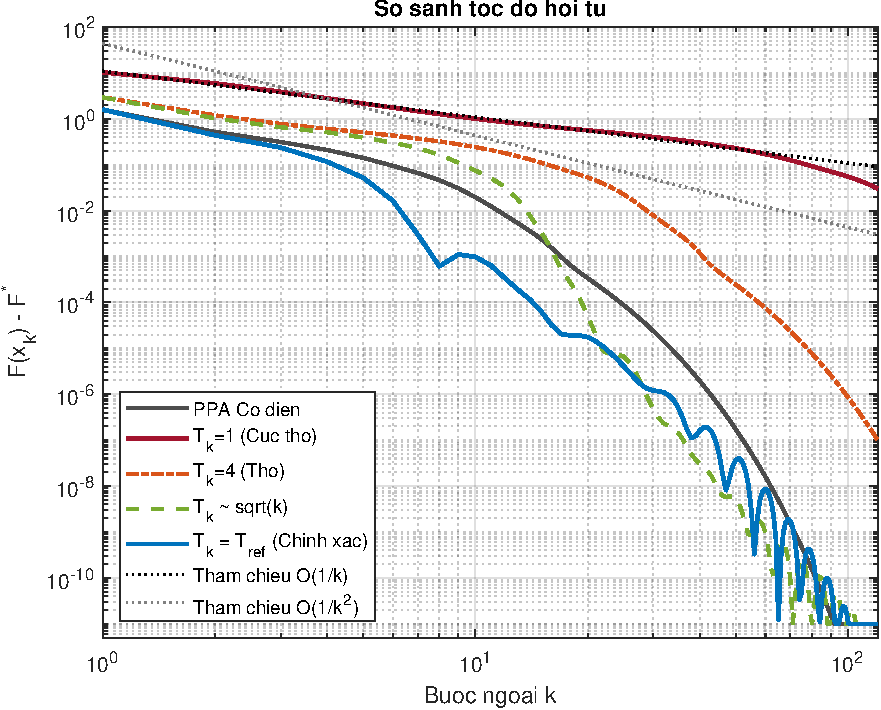
\includegraphics[width=0.8\linewidth]{figures/convergence-comparison.pdf}
    \caption{So sánh tốc độ hội tụ của thuật toán PPA cổ điển và các biến thể ứng với các lịch trình \(T_k\) khác nhau. Kết quả thực nghiệm cho thấy lịch trình \(T_k \sim \sqrt{k}\) duy trì tốc độ hội tụ \(O(1/k^2)\), gần như tương đương với trường hợp giải chính xác (\(T_k = T_{\mathrm{ref}}\)), đồng thời giúp giảm đáng kể chi phí tính toán.}
    \label{fig:conv-comparison}
\end{figure}
\begin{figure}[H]
    \centering
    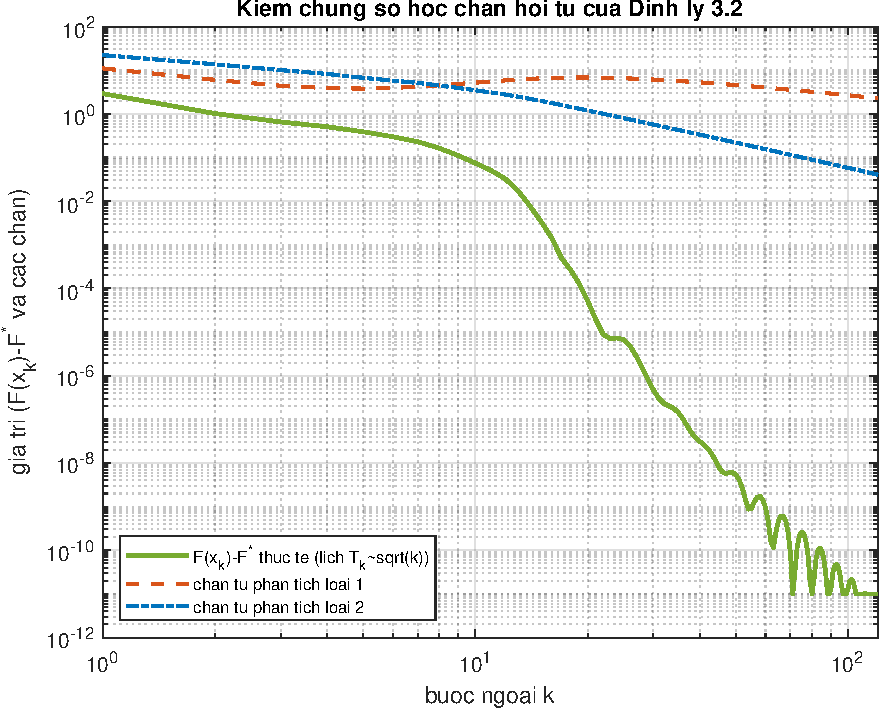
\includegraphics[width=0.8\linewidth]{figures/bound-verification.pdf}
    \caption{Kiểm chứng số học các chặn hội tụ của Định lý~\ref{thm:estimate-main}. Đồ thị log-log biểu diễn khoảng cách của hàm mục tiêu $F(x_k) - F^*$ (đường liền nét màu xanh lá) theo các bước lặp ngoài $k$, được so sánh với chặn lý thuyết Loại 1 (đường đứt nét màu cam) và chặn lý thuyết Loại 2 (đường gạch chấm màu xanh dương). Kết quả thực nghiệm cho thấy với lịch trình vòng lặp nội $T_k \approx \sqrt{k}$, thuật toán hội tụ nhanh hơn và chặt chẽ hơn nhiều so với dự đoán của các giới hạn lý thuyết, và đi ngang ở ngưỡng $10^{-11}$ do giới hạn độ chính xác của máy tính (sàn nhiễu).}
    \label{fig:bound-verification}
\end{figure}
\begin{figure}[H]
    \centering
    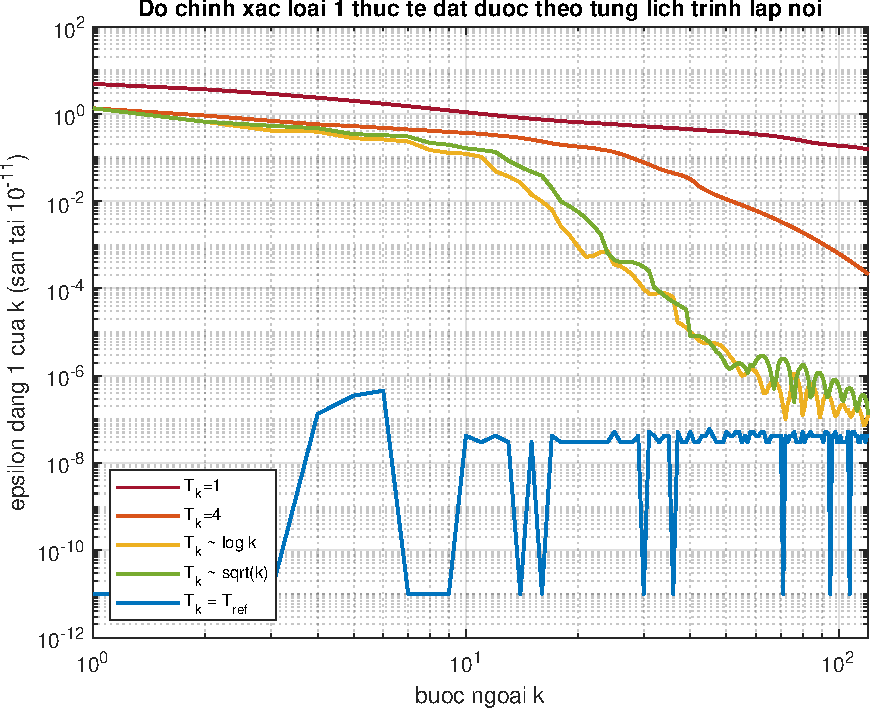
\includegraphics[width=0.8\linewidth]{figures/type1-accuracy.pdf}
    \caption{Sự suy giảm của sai số Loại 1 ($\epsilon_k$) theo số bước lặp ngoài $k$ dưới các kịch bản chọn số vòng lặp nội $T_k$ khác nhau. Biểu đồ log-log cho thấy các chiến lược tăng dần $T_k$ theo bước lặp, cụ thể là $T_k \sim \log k$ (đường màu vàng) và $T_k \sim \sqrt{k}$ (đường màu xanh lá), giúp sai số hội tụ nhanh chóng và đạt hiệu quả cao. Ngược lại, việc cố định $T_k$ ở mức thấp ($T_k=1$ hoặc $T_k=4$) khiến sai số giảm rất chậm. Lịch trình tính toán gần đúng chính xác ($T_k = T_{ref}$, đường màu xanh dương) nhanh chóng dao động quanh mức giới hạn sàn nhiễu số học của máy tính ($10^{-11}$).}
    \label{fig:eps-decay}
\end{figure}
\end{essayonly}
\begin{slidesonly}
    \begin{figure}[H]
    \centering
    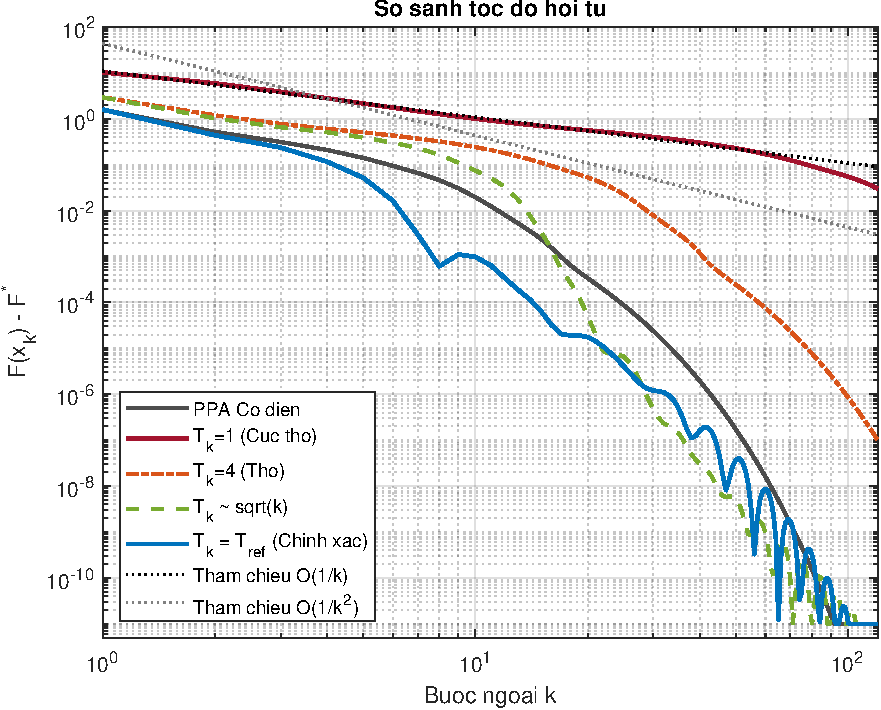
\includegraphics[width=0.9\textwidth, height=0.9\textheight, keepaspectratio]{figures/convergence-comparison.pdf}
    \label{fig:conv-comparison-slide}
\end{figure}
\end{slidesonly}
    \end{frame}
    \begin{frame}[plain]{Tài liệu tham khảo}
        \bibliographystyle{unsrtnat}
        \bibliography{refs}
    \end{frame}
\end{document}